% You should title the file with a .tex extension (hw1.tex, for example)
\documentclass[11pt]{article}
\usepackage{hyperref}
\usepackage{bmpsize}
\usepackage[pdftex]{graphicx}
\usepackage{amsmath}
\usepackage{amssymb}
\usepackage{amsthm}
\usepackage{fancyhdr}
\usepackage[margin=2.5cm]{geometry}
\newcommand{\Ohm}{\Omega}
\newcommand{\inv}{^{-1}}
\newcommand{\snrin}{\text{SNR}_{in}}
\newcommand{\snrout}{\text{SNR}_{out}}
\renewcommand{\part}[1] {\vspace{.10in} {\bf (#1)}}


\pagestyle{fancyplain}


\begin{document}
\title{Building an Amplifed FM Radio and Measuring Noise}
\author{David Galbraith}
\maketitle
%COMMENT: In Latex, using the maketitle function will perform all the formatting
%you had set up in the code below in a standard fashion

\normalsize
\begin{abstract}
For this lab, we made an FM radio that took a frequency-modulated signal and turned it
into music. Then, we made an amplifier that made the music louder. Finally, we tried to use
amplification to get measurements of Johnson-Nyquist noise, and we wrote Python programs
to verify the Central Limit theorem and the change in standard deviation with
increasing sample size. Along the way, we measured the velocity of propagation of 
electrical signals in wires, getting $1.9*10^8$ meters per second, and we measured the impedance
of our cables as $50 \Omega$. 
\end{abstract}
%COMMENT: It is customary to use the abstract environment for the
%abstract, and to not include a pagebreak after the abstract prior to
%the introduction in a scientific paper


\lhead{\fancyplain{}{\textbf{Lab 1}}}      % Note the different brackets!
\rhead{\fancyplain{}{David Galbraith}}
\medskip                        % Skip a "medium" amount of space
                                % (latex determines medium is)
                                % Also try: \bigskip, \littleskip

\thispagestyle{plain}
 

\section{Introduction}
%COMMENT: Sections and subsections have their own format that will make
%the divisions in what you wrote more clear, and will number themselves,
%allowing you to focus more on content rather than order

FM demodulation is a way of extracting information encoded in an electrical signal. To interpret a signal, 
we use frequency filtering and envelope detection. The filter we used was a bandpass filter, because
we only wanted frequencies in the vicinity of 1.045 MHz, because that was the frequency at which the
relevant signals were being transmitted, and everything else was just noise. A bandpass filter only
lets through frequencies around its ``resonant frequency'', which can be calculated from the formula
$\omega = (2\pi\sqrt{LC})\inv$, where $\omega$ is the resonant frequency, $L$ is
the inductance of the inductor in Henrys, and $C$ is the capacitance of
the capacitor in farads. Another relevant number for a filter is the bandwidth. The
bandwidth gives a measurement of the range of frequencies the filter allows through. 
One half-bandwidth above and below the resonant frequency, the output of the filter 
is $70.7\%$ of the input. More than one half-bandwidth above and below resonance, the output
rapidly drops off; less than one half-bandwidth above and below, it is closer to 1 times the input.
The bandwidth of an LC filter is given by $\Delta f = (2\pi RC)\inv$ where $R$ is a resistance
that precedes the LC subcircuit. 

In building the amplifier, we also used transistors. Transistors are very important because they are what
computers are made of among other reasons. In circuits, transistors act as switches and amplifiers. They have
three pins: the collector, the base, and the emitter. When current is flowing into the base, the transistor
amplifies the current flowing through the collector and emitter voltages. When current is not flowing into the base,
it is as if there is an open circuit between the collector and emitter pins. The base voltage $V_{BE}$ is the 
voltage between the base and emitter pins. 

\section{Experiments, Observations, Analysis and Interpretation}

In the first part of the lab, the first thing we did was make capacitive and resistive voltage dividers, the
structure of which you can see in Figure \ref{RC_div}.
\begin{figure}
\centering
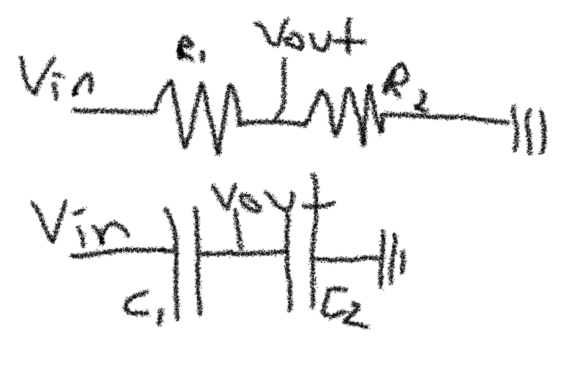
\includegraphics[scale=0.35]{dividers}
\caption{Resistive and capacitive voltage dividers \label{RC_div}}
\end{figure}
%COMMENT: Using \label{value} and \ref{value} will allow you to refer to
%a specific figure without worrying about the order in which you have
%them in your document. While this obviously matters somewhat in terms
%of the logical flow of you paper, it's really helpful if you're moving
%things around as you write your paper. I did this for the first figure,
%but you can change the rest fairly easily. Additionally, \centering
%will put the figure in the middle of the page when you scale it down to
%a more reasonable size.
A resistive voltage divider dissipates through its component resistors a voltage amount proportional to
their resistance, operating in the same way under AC and DC conditions. A capacitive voltage divider 
blocks DC current, and it dissipates through each capacitor an amount of voltage proportional to its
capacitance when AC current is input. Our resistors and capacitors were equal in strength, so the output 
voltage was half the input voltage for both dividers. In Figure \ref{VDs}, you can see an oscilloscope reading 
of the input and output voltage of our resistive voltage divider and a similar reading
for the capacitive one. 
\begin{figure}
\centering
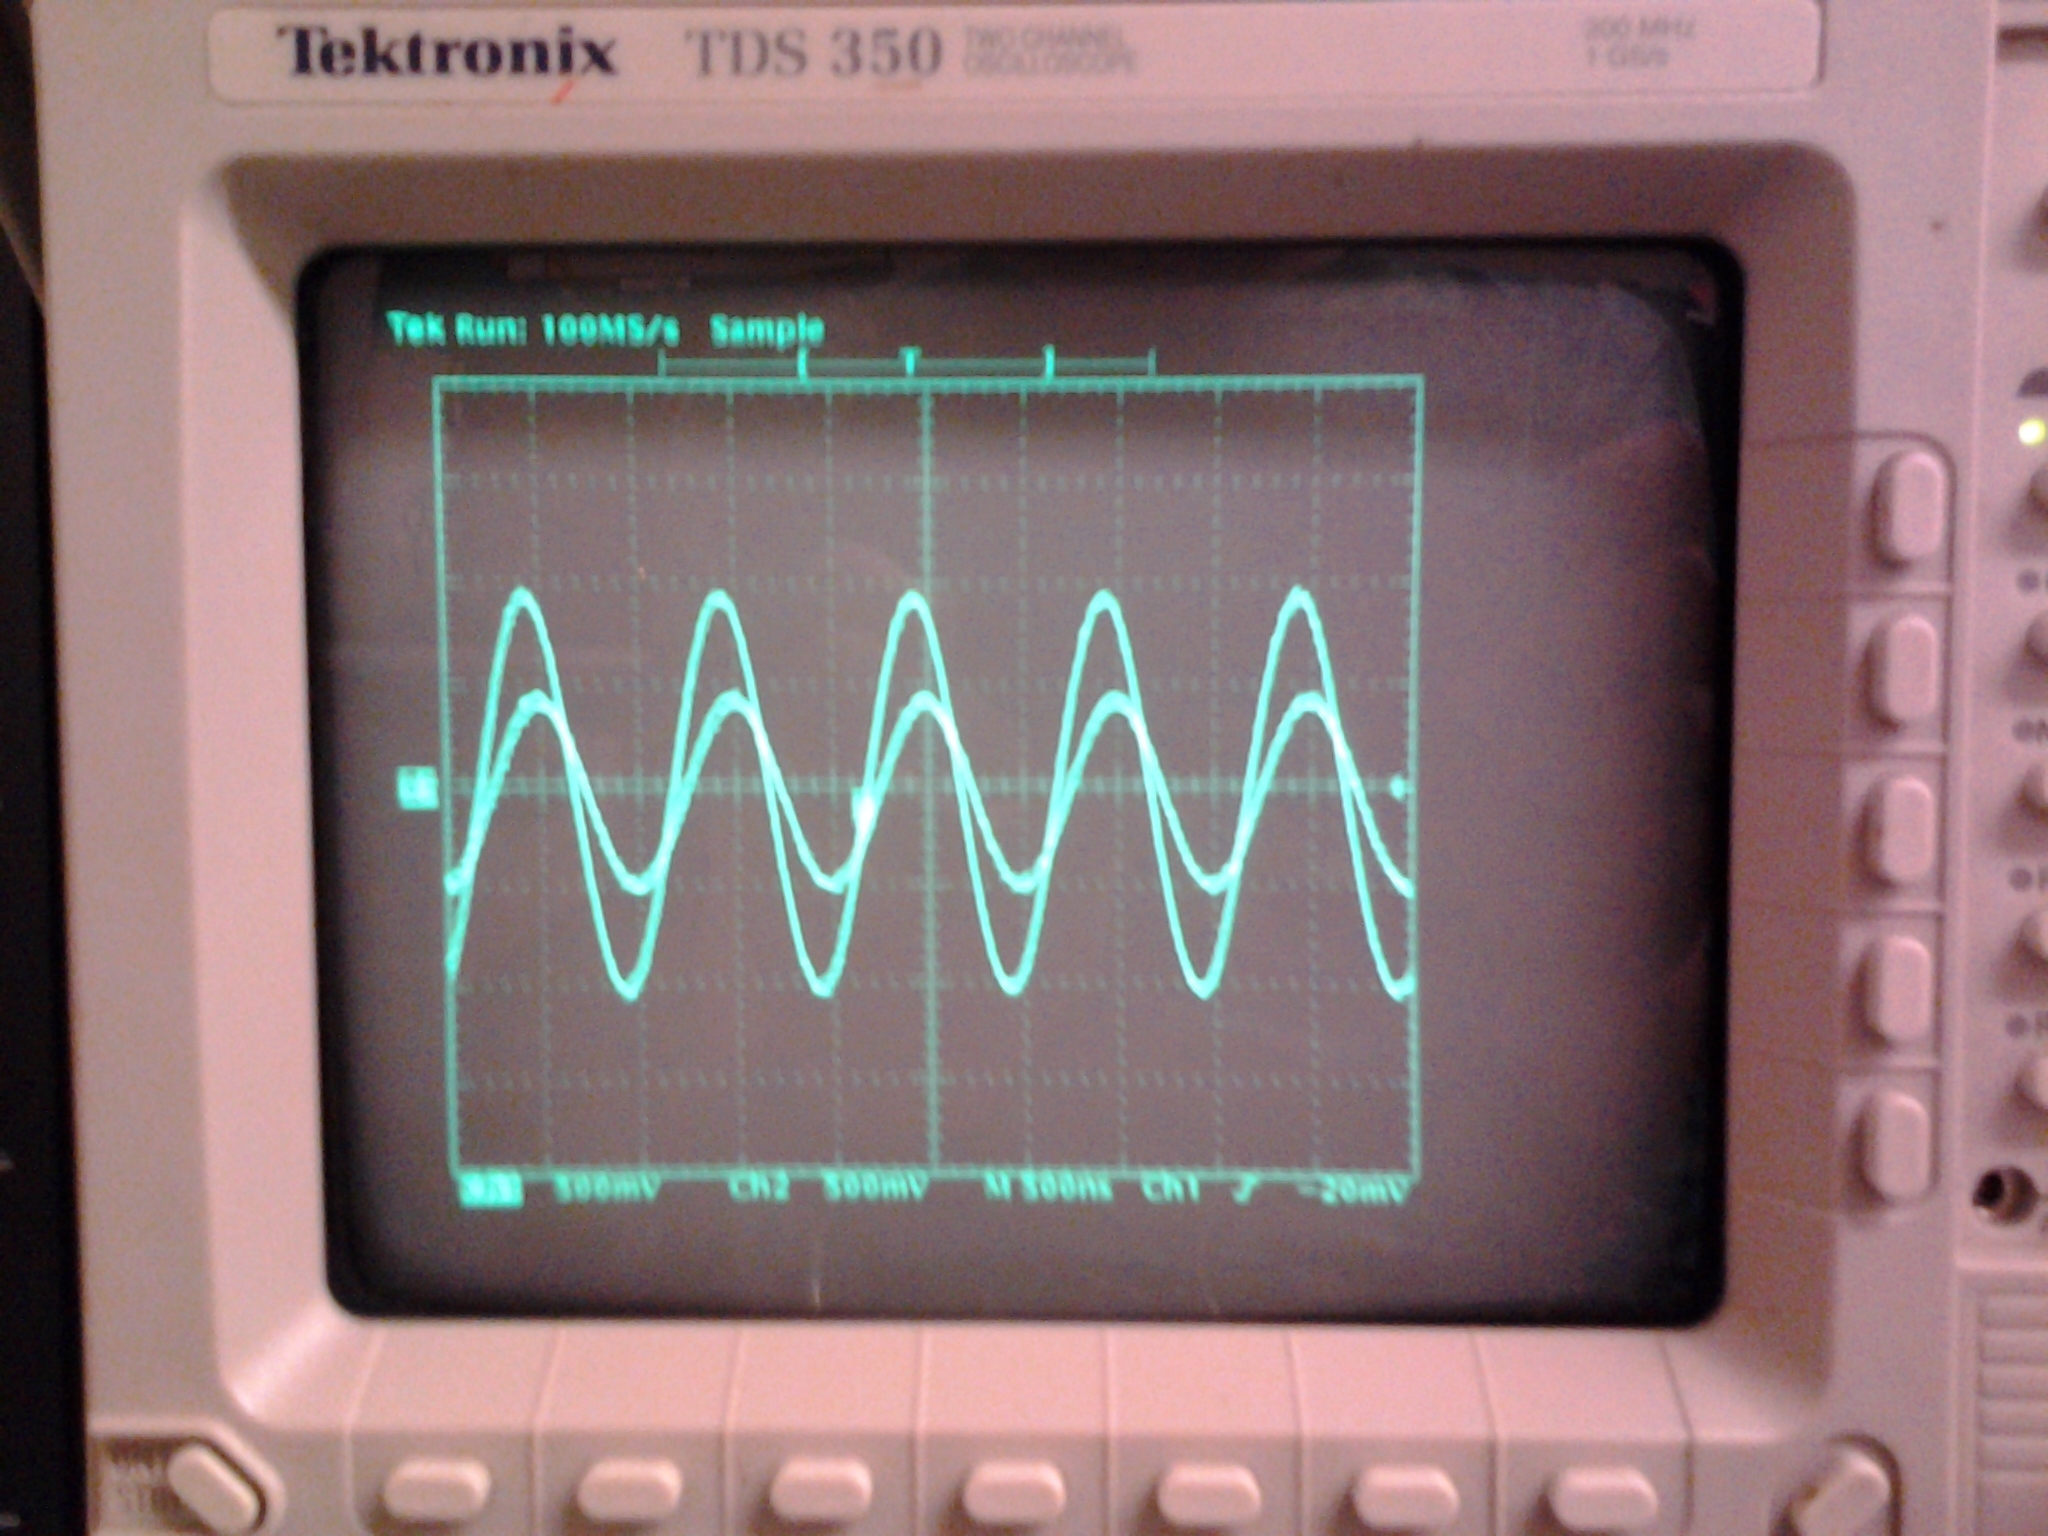
\includegraphics[scale=0.1]{vd}
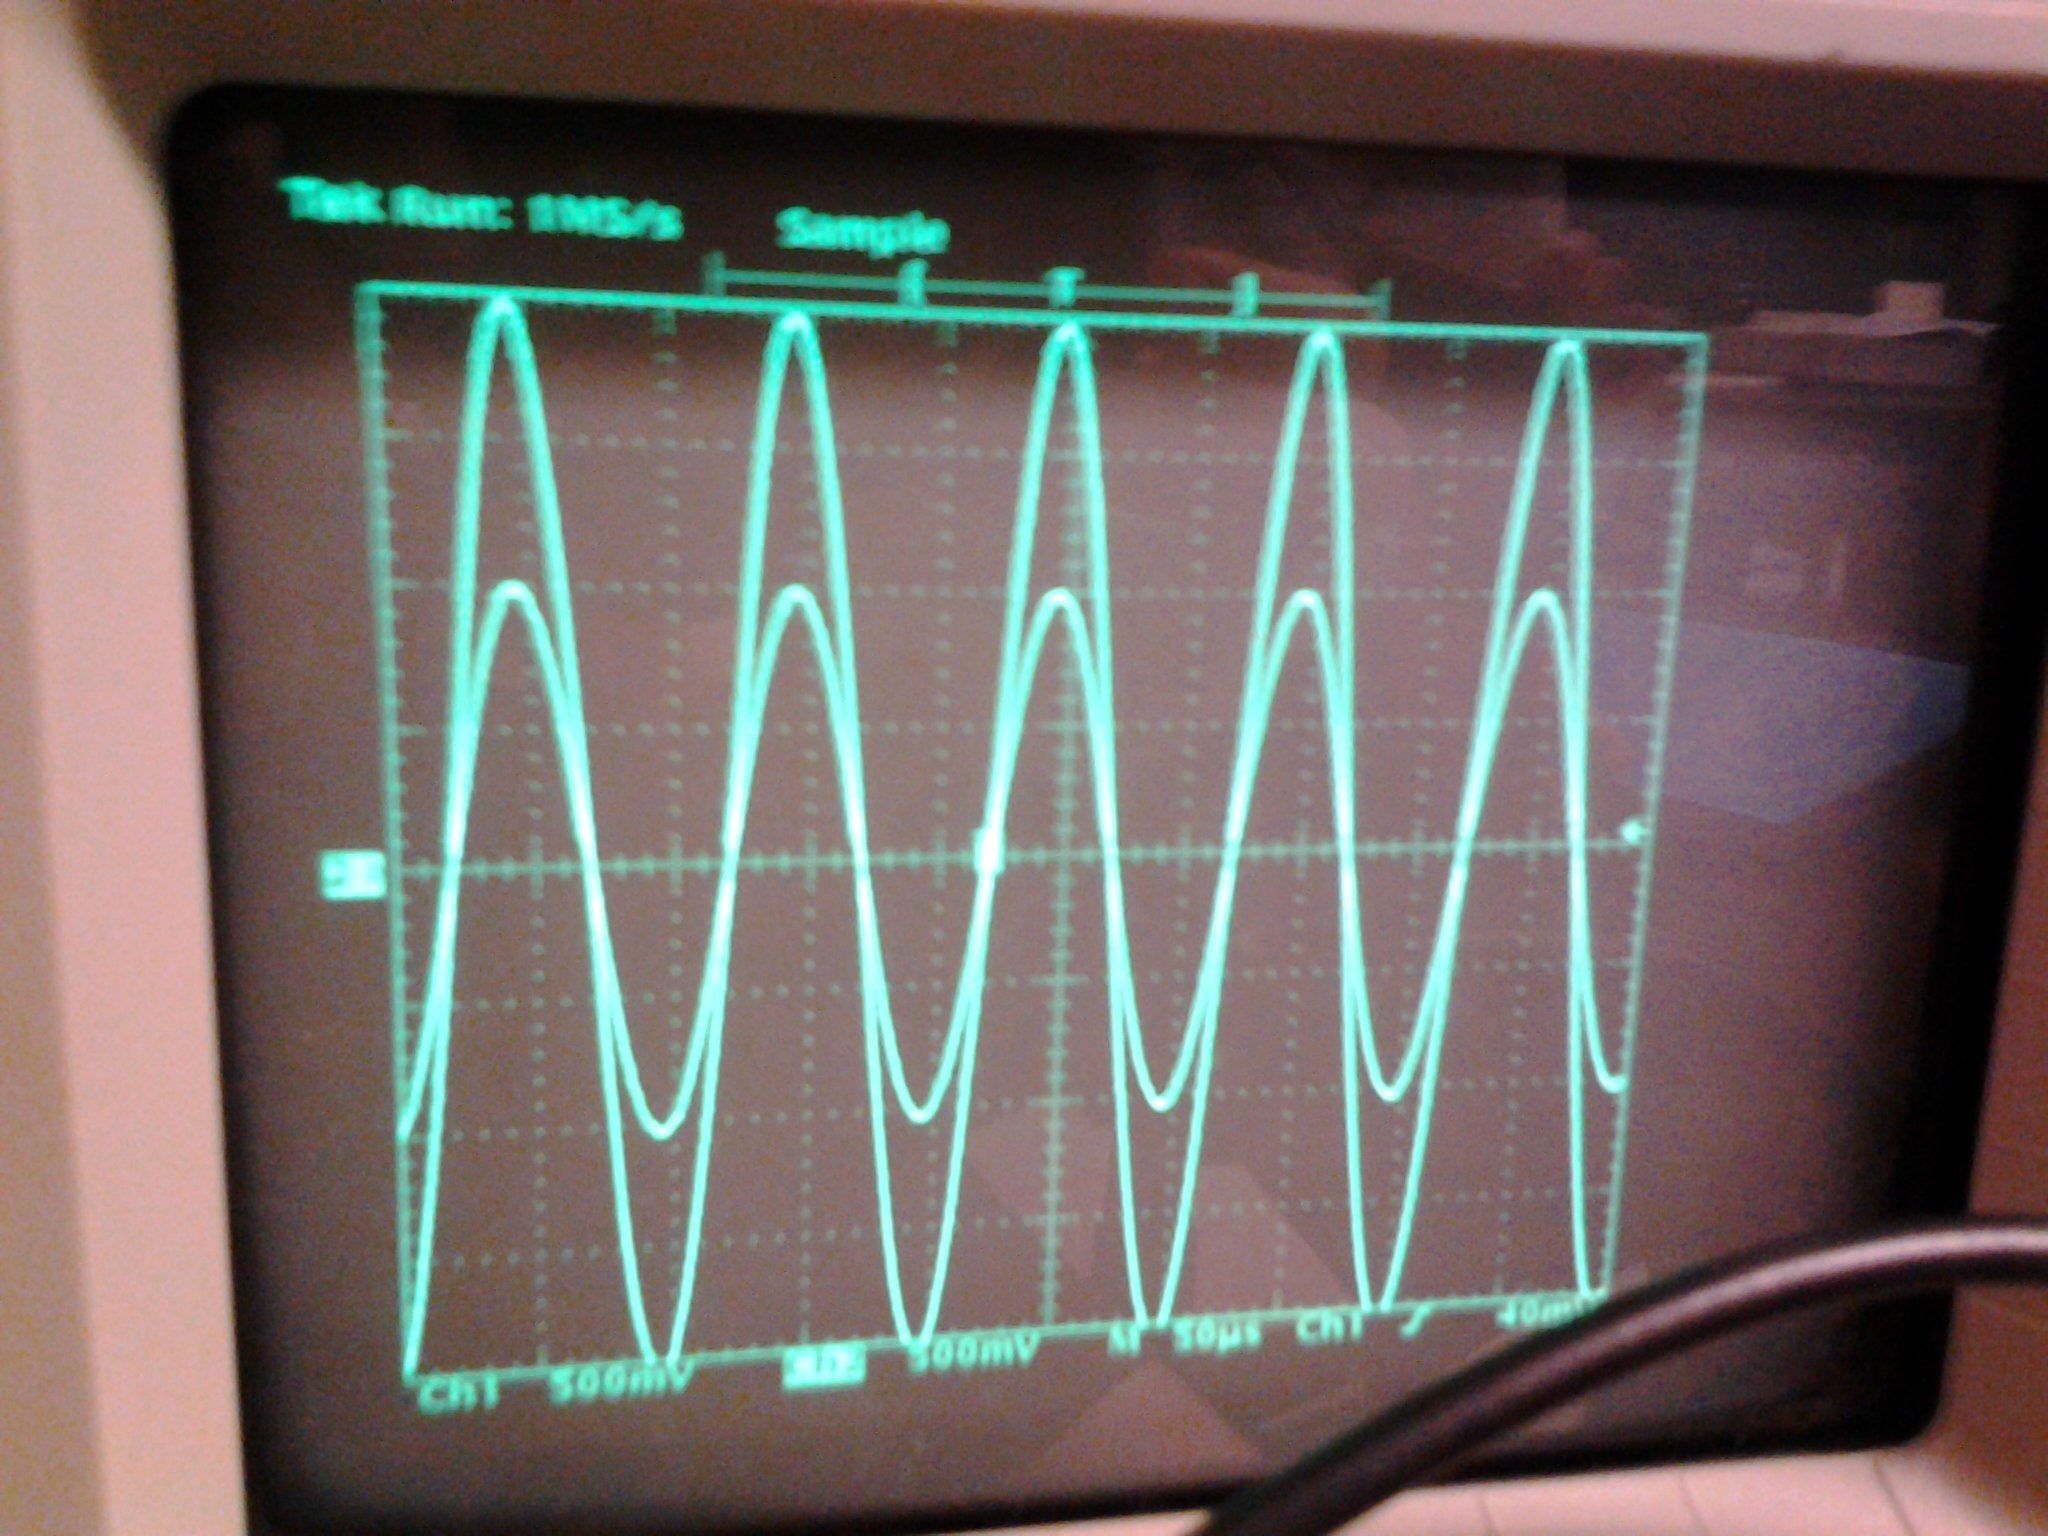
\includegraphics[scale=0.1]{photo1}
\caption{Left: $V_{in}$ and $V_{out}$ for a resistive voltage divider; Right:$V_{in}$ and $V_{out}$ for a capacitive voltage divider \label{VDs}}
\end{figure}
%COMMENT:By placing your figures in the flow of your text, you can
%increase the likelihood that they appear in reasonable places based on
%where you reference them. Combining figures (2 & 3 were combined) that
%are related or demonstrate two aspects of one thing can also allow you
%to use space in your paper more effectively.
Next, we made low-pass and high-pass filters with cutoffs close to 100 kHz. A low-pass filter can be seen in Figure \ref{LPFD}, together with its theoretical output.
\begin{figure}
\centering
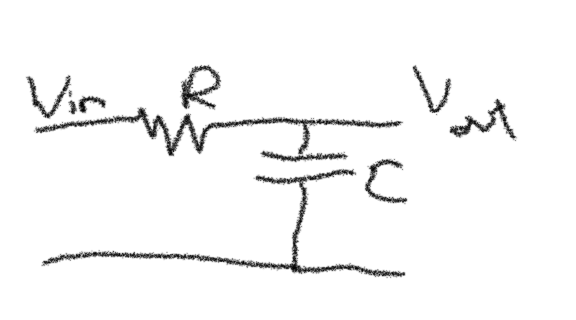
\includegraphics[scale=0.3]{lpcircuit}
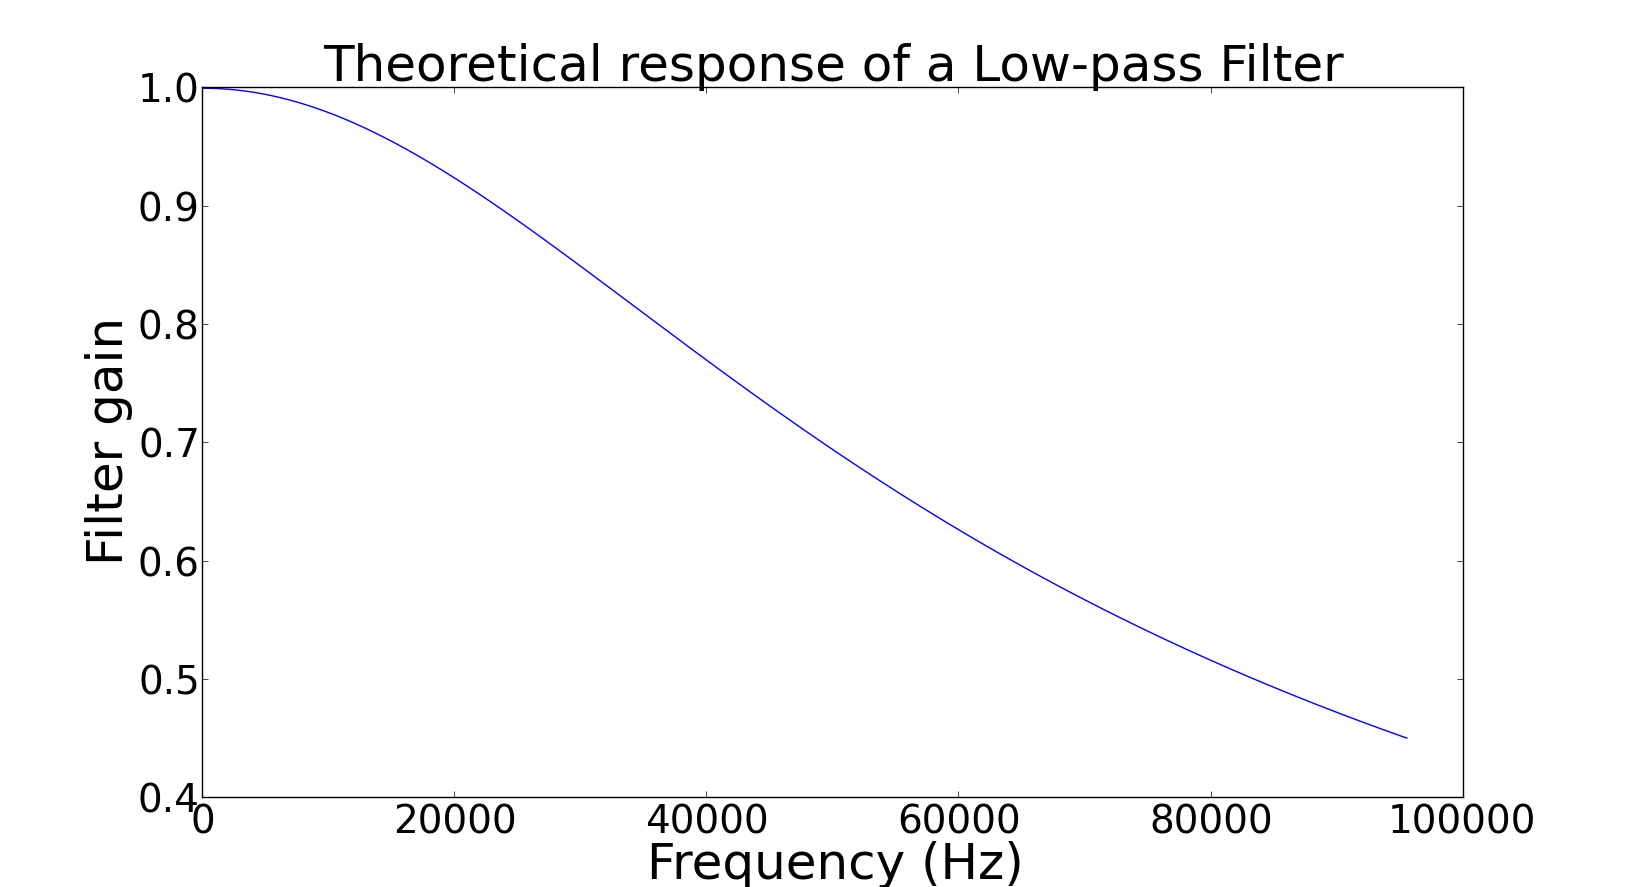
\includegraphics[scale=0.25]{lowpass}
\caption{Design and Response of a Low-pass Filter \label{LPFD}}
\end{figure}
%COMMENT: Increase the font size in the second plot in this figure, and
%decrease the size of the figure (I decreased the size of the figure but
%did not increase the font size)
 We used a resistance of 160 $\Omega$ and a capacitance of 10000 pF, so the
cutoff frequency of our low-pass filter was $(2\pi RC)\inv = 99472$ Hz, close to 100 kHz. In Figure \ref{LPFR}, you can see a
plot of the output voltages we measured for input voltages of varying frequencies:
clearly, it basically matches the theoretical distribution. 
\begin{figure}
\centering
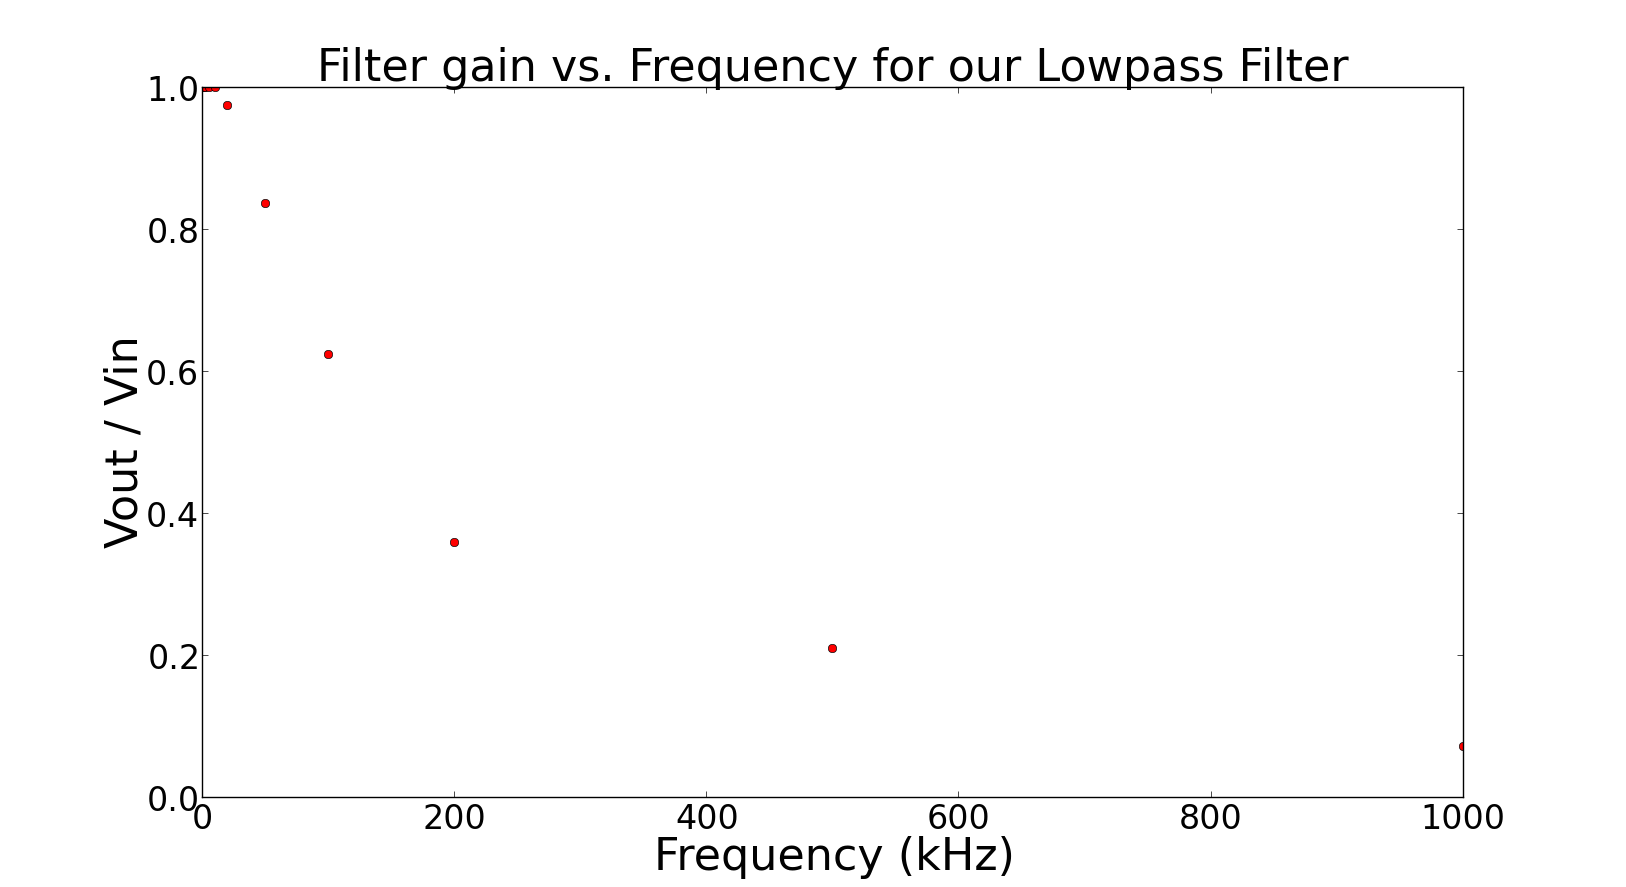
\includegraphics[scale=0.3]{lpresplot}
\caption{Plot of Measured Low-Pass Filter Effects \label{LPFR}}
\end{figure}
In Figure \ref{HPFD}, you can see a high-pass filter
along with its theoretical output: a high-pass filter attenuates small frequencies and is passable to high frequencies.
\begin{figure}
\centering
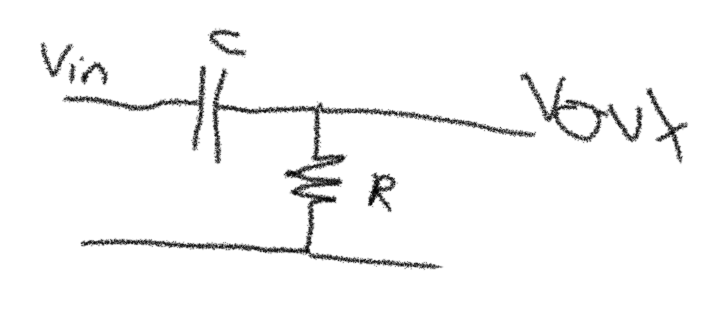
\includegraphics[scale=0.25]{hpcircuit}
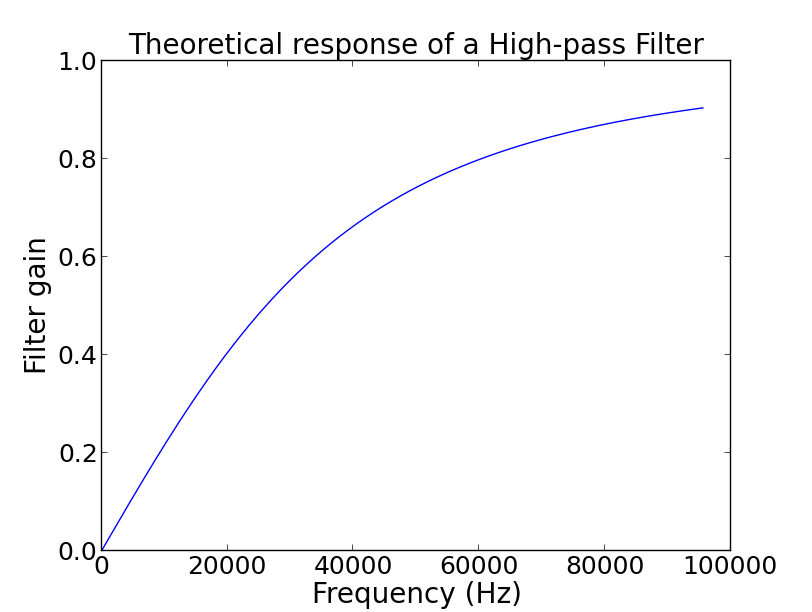
\includegraphics[scale=0.4]{highpass}
\caption{Design and Response of a High-Pass Filter \label{HPFD}}
\end{figure}
We used the same components for this circuit as for the low-pass filter, so it has the same cutoff frequency.
Figure \ref{HPFR} gives a plot of the input and output voltages we measured for this filter. 
\begin{figure}
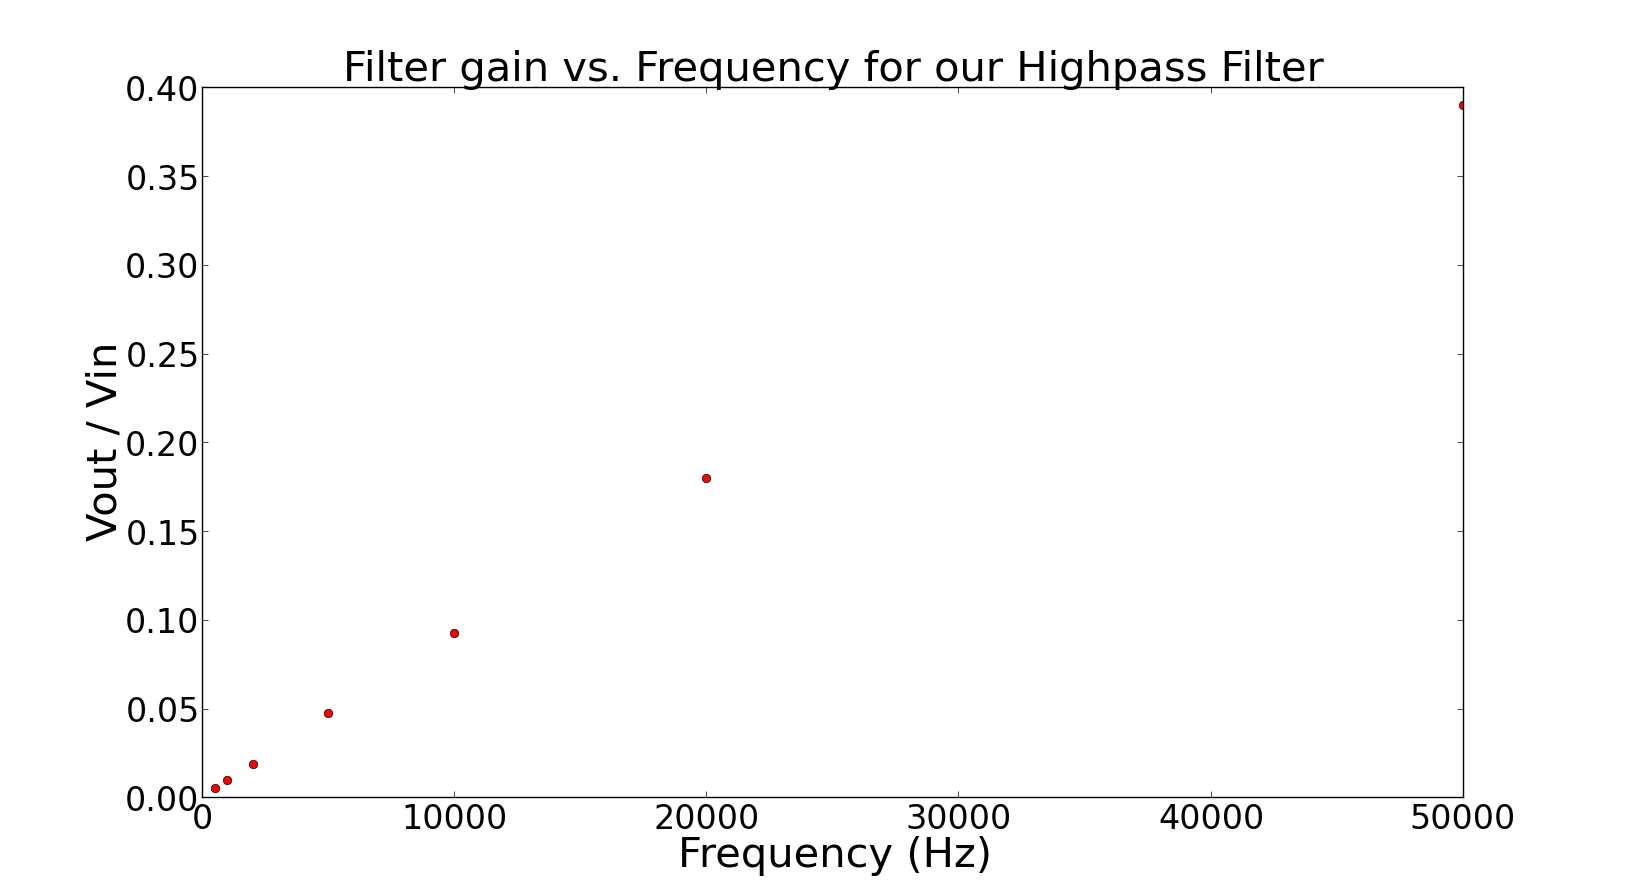
\includegraphics[scale=0.3]{hpresplot}
\caption{Plot of Measured High-Pass Filter Effects \label{HPFR}}
\end{figure}
%COMMENT: Captions should go below figures always.

Next, we made a few circuits with diodes. A diode only allows current to flow in one direction, so if you give it AC
input, it will output DC. First, we made a simple circuit of just a resistor and a diode to measure the voltage drop
across a conducting diode as a function of input current. Then, we 
sent in a large oscillating signal and viewed the DC output of the diode on an oscilloscope: a picture of that appears
in Figure \ref{OSCI}. 
\begin{figure}
\centering
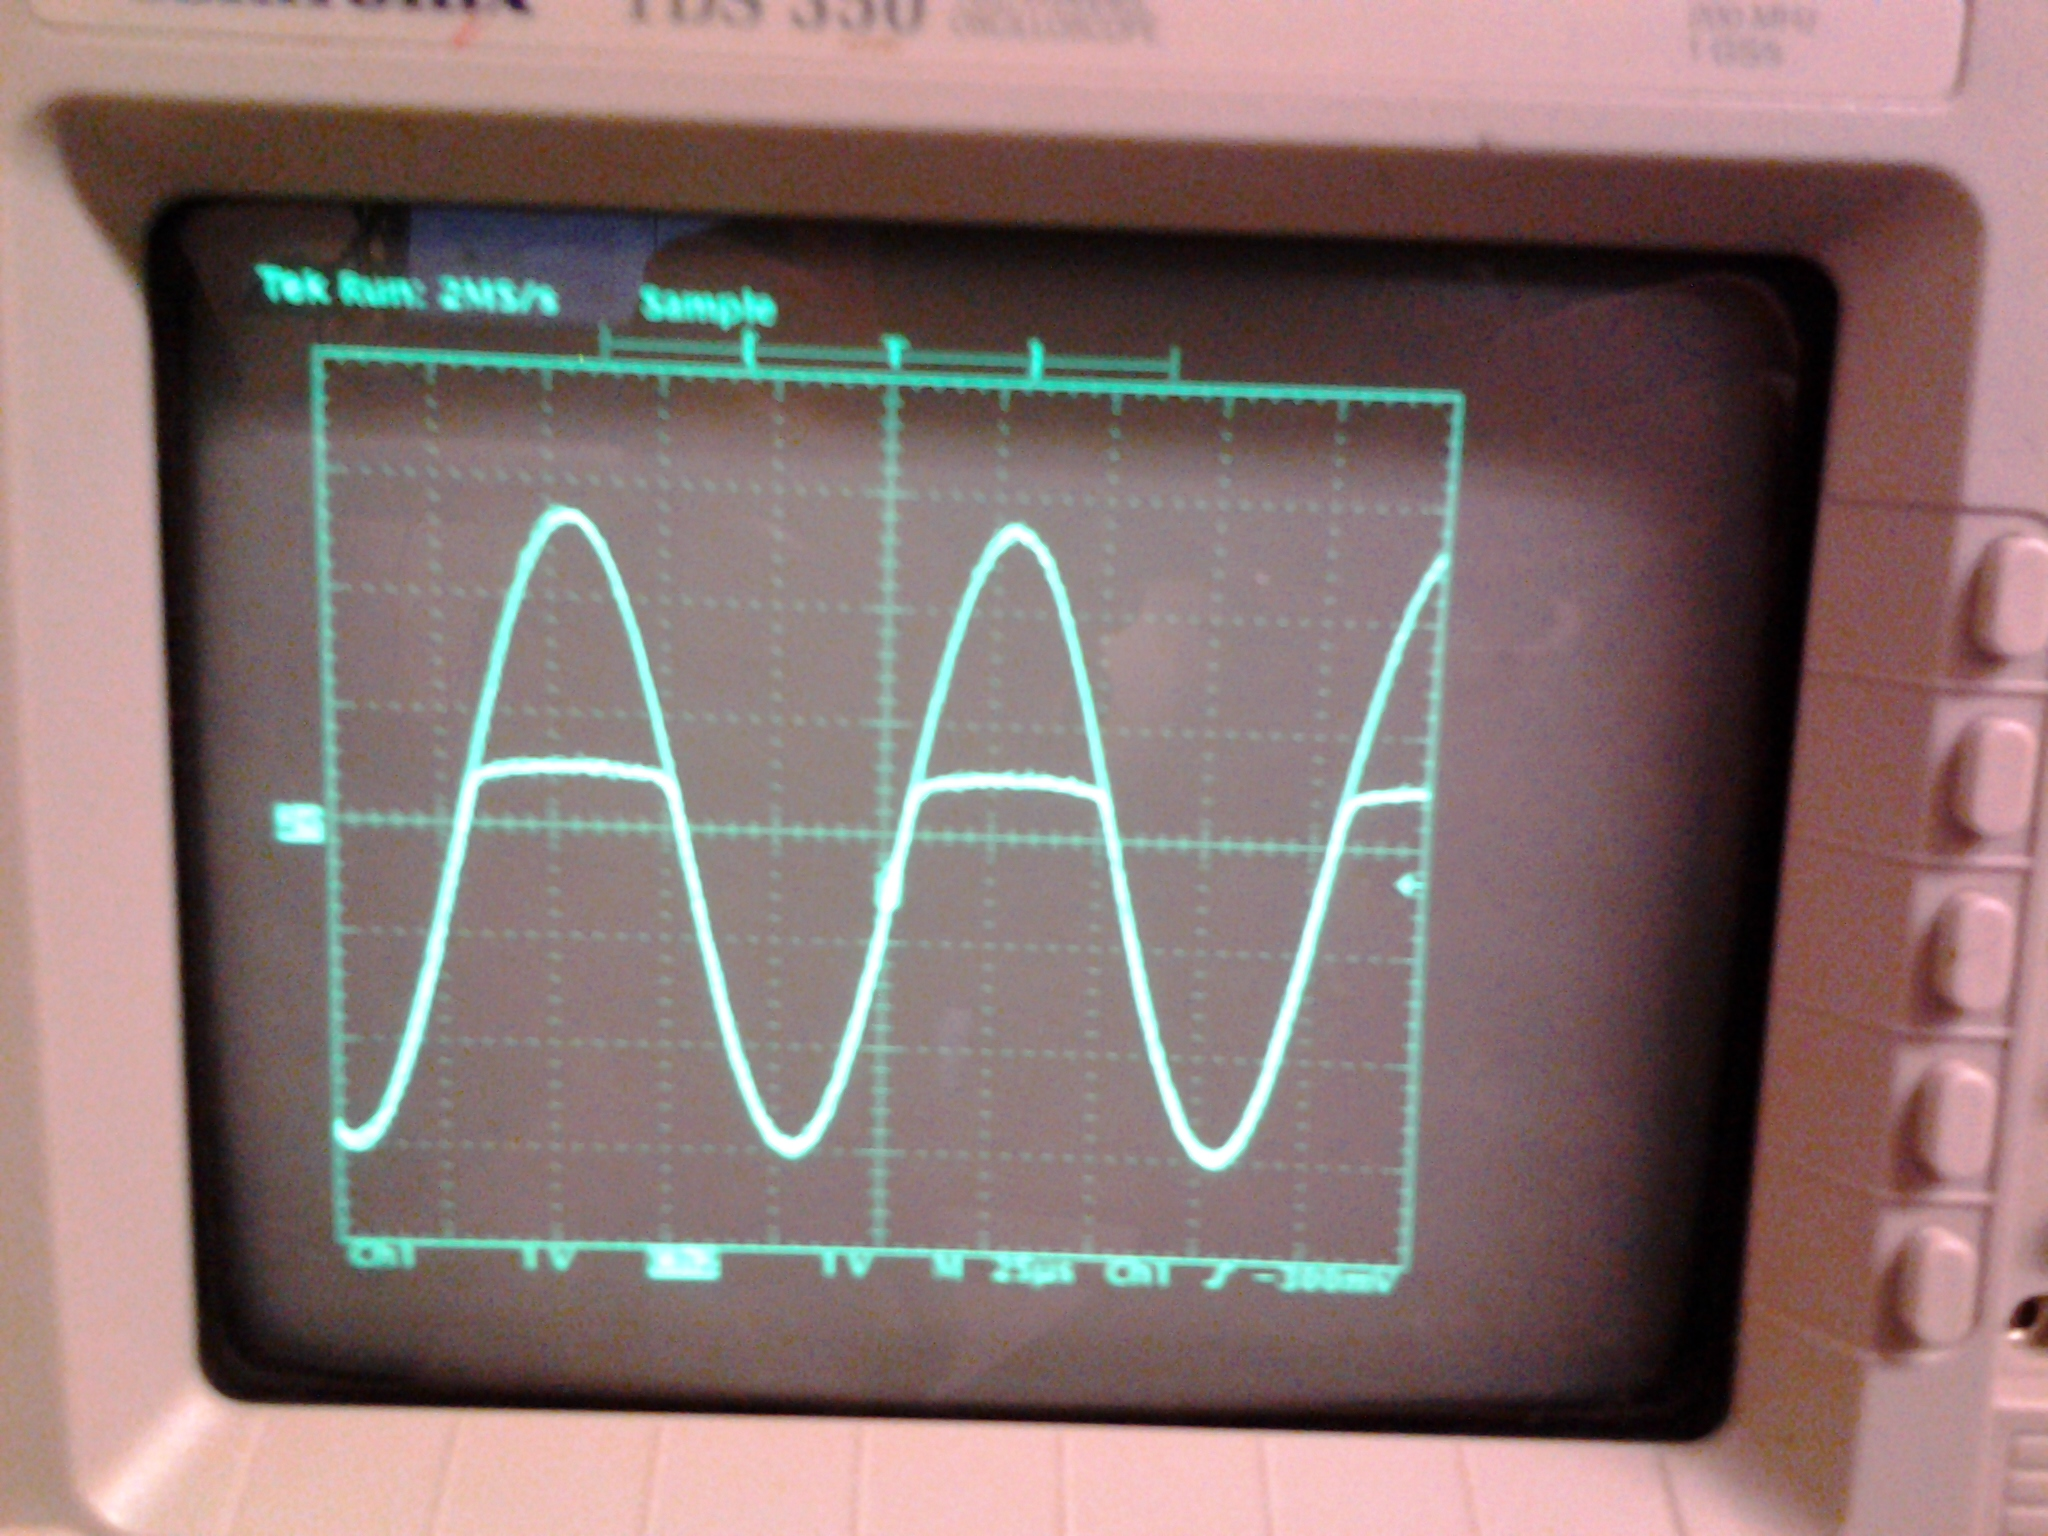
\includegraphics[scale=0.1]{diode}
\caption{Oscilloscope view of diode given AC \label{OSCI}}
\end{figure}

Finally, we got around to building our FM Demodulation Circuit, which
you see in Figure \ref{FMDEMOD}.
\begin{figure}
\centering
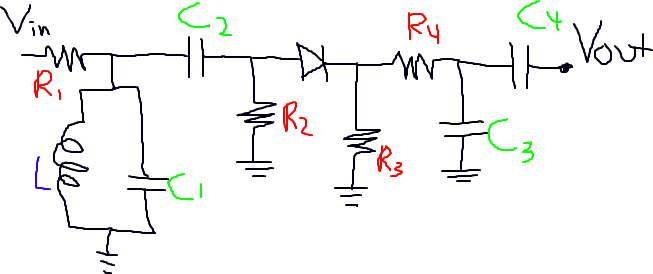
\includegraphics[scale=0.6]{circuit}
\\ 
$R_1 = 33 \Ohm; R_2 = 150\Ohm, R_3 = 150 \Ohm, R_4 = 150 \Ohm, L = 1 \mu$H$; C_1 = 22000$ pF$; C_2 = C_3 = C_4 = 10000$ pF.
\\
\caption{FM Demodulation Circuit \label{FMDEMOD}}
\end{figure}

\begin{figure}
\centering
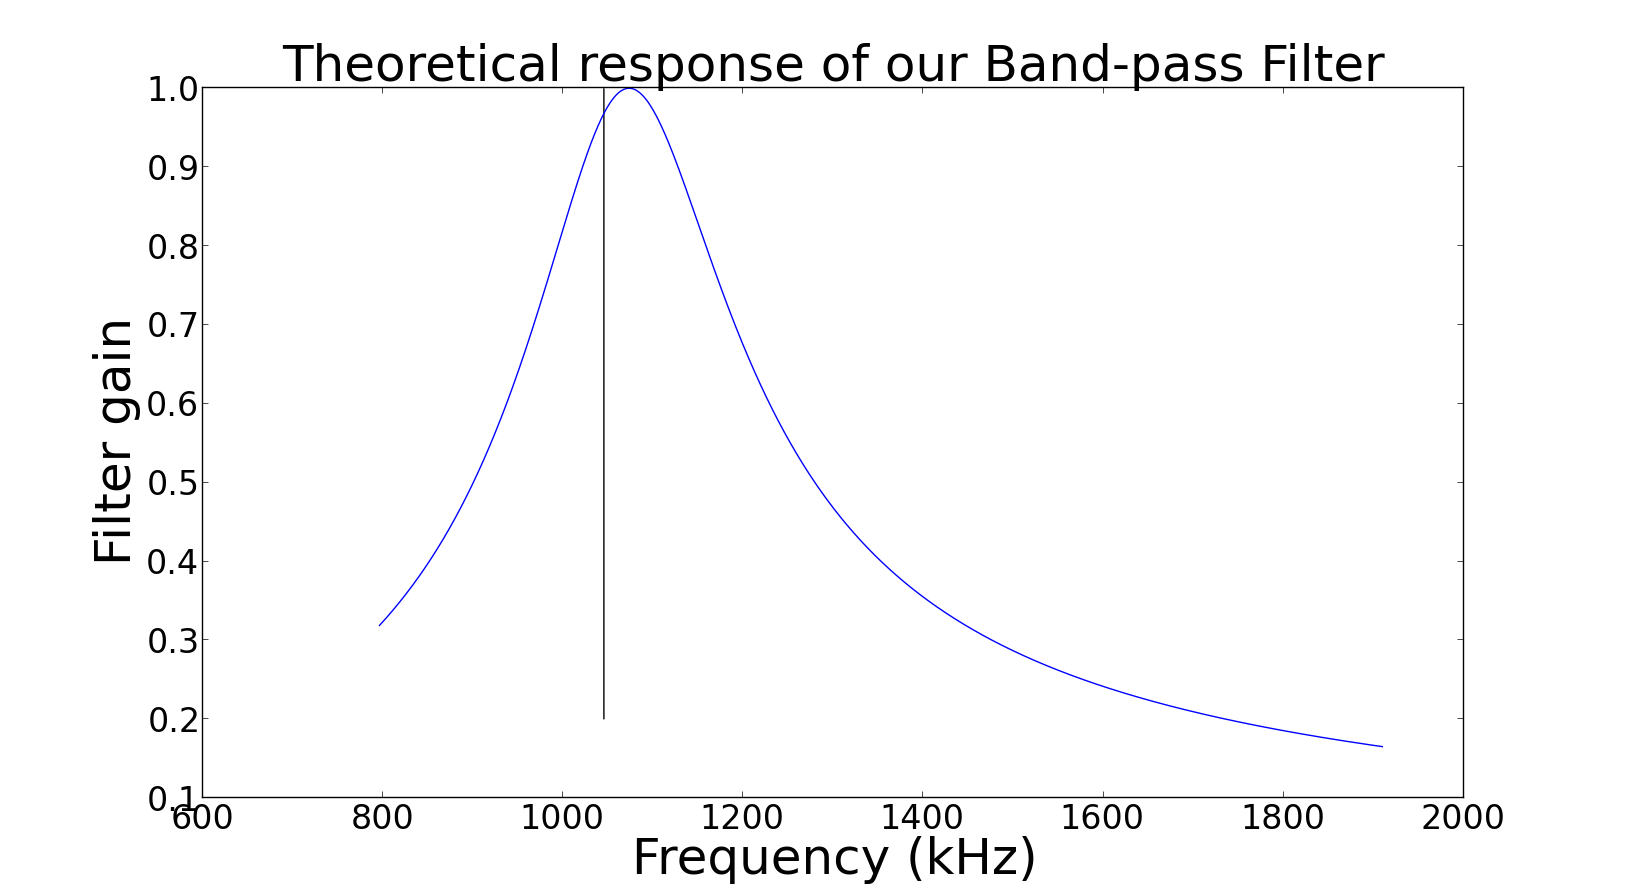
\includegraphics[scale=0.3]{bandpass}
\caption{Calculated transfer function for our bandpass filter \label{BP}}
\end{figure}
On the far left you see $V_{in}$, which is where the signals come in
from the source. Then to the right of that there is a bandpass filter
consisting of $L$ and $C_1$. The LC bandpass filter for this circuit is
centered at roughly 1 MHz using an inductance of 1 $\mu$H and a capacitance of 22000 pF, giving a resonant frequency of $(2\pi
\sqrt{LC_1})\inv = 1.073$ MHz. This was the closest we could get to the
1.045 MHz bandwidth of the input signal with the available
materials. Its bandwidth is $(2\pi R C)\inv$ = 202 kHz. Since the input signal is well within this range of the filter's
resonant frequency, it comes through strongly. 
\begin{figure}
\centering
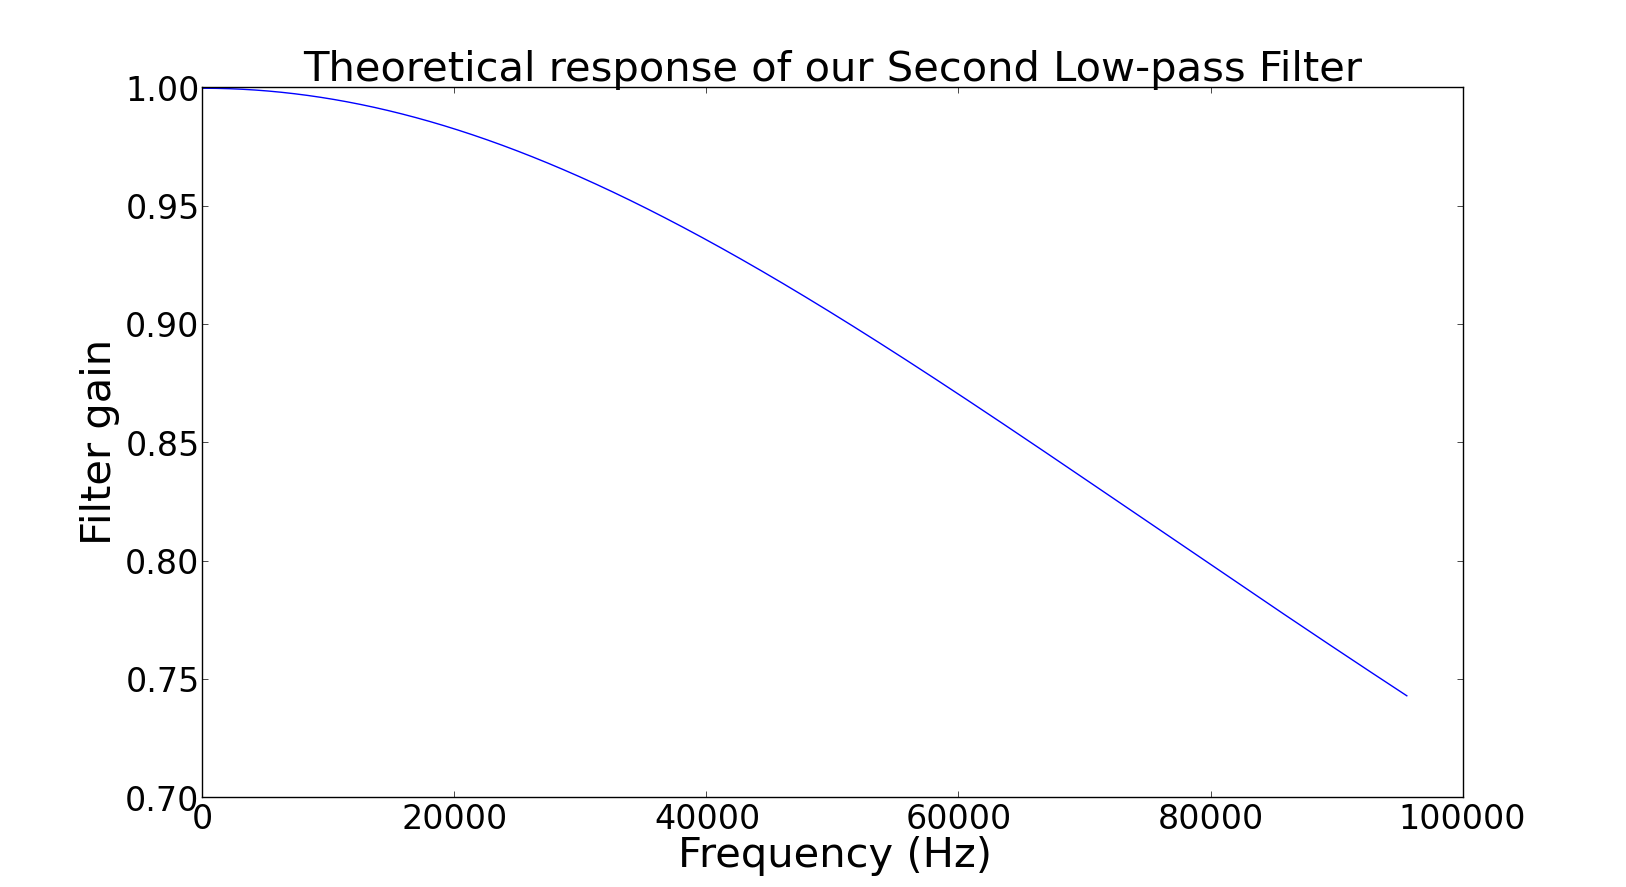
\includegraphics[scale=0.3]{lowpass2}
\caption{Transfer function for our low-pass filter \label{TFLP}}
\end{figure}
A plot of its
expected output as a function of frequency appears in Figure \ref{BP}. The vertical
line indicates 1.045 MHz, the frequency of the input signal. 
%COMMENT: In a report you don't need to write out unit names, and it
%would actually be preferred you use things like $\mu$H versus microhenry
\\

Also on the left side of the circuit but not a part of the bandpass filter, we have $R_1$ 
and $C_2$. These components are used for biasing, which is when you optimize
a signal to work with a certain device. $R_1$ decreases the amplitude of the input signal,
because that is what resistors in alternating currents do, while $C_1$ puts a phase
shift between the voltage and current of the input signal, because that is what capacitors
in alternating currents do. These changes to the signal help it work properly with the diode.
The value of $C_1$ was fixed $a$ $priori$ by the fact that 10000 pF was the only capacitance
value we had available, having already used our only 22000 pF capacitor in the LC filter. 
We found a usable value for $R_1$ by trial and error, putting in every resistor value we had
until the circuit worked. $R_2$ serves to discharge the input current when the diode is functioning
as an open circuit; its value can be chosen arbitrarily as long as it can actually discharge the
voltage efficiently enough that the circuit does not catch fire.
\\

The remainder of the circuit serves as an envelope detector. An envelope detector
takes a high-frequency signal as input and sends to the output the envelope of that signal.
The envelope of an oscillating signal is basically the curve given by connecting the
peaks of each of its waves. This circuit works as an envelope detector because the diode 
only allows current to flow in the direction that it is pointing on the diagram. When current
is flowing through the diode, it acts like a short
circuit, so the output signal of the diode is equal to its input signal. At other times, its output signal
is zero. A ``textbook'' envelope detector consists only of the diode, $R_3$, and $C_3$, so only
consider those parts for the moment. When the diode is acting as a short circuit, its output
is a DC signal whose voltage equals the amplitude of the input voltage;
under these conditions, this voltage accumulates on $C_3$. When the diode is
acting like an open circuit, $C_3$ discharges through $R_3$, so $V_{out}$ drops until
the diode goes back to letting charge through. As a result of this process, $V_{out}$ is an AC 
signal that measures the amplitude of $V_{in}$. That's why it's called an ``amplitude-modulated signal''. 
The combination of $R_4$ and $C_3$ acts as a low-pass filter on this signal, since the amplitude of the
input might oscillate due to thermal noise or some other high-frequency source, but the major fluctuations
in the amplitude that we are trying to measure happen with lower frequency. The cutoff frequency for the
low-pass filter is $(2\pi\sqrt{R_4C_3})\inv \approx$ 106 kHz. Its transfer function is plotted in Figure \ref{TFLP}.
Cutoff frequency is also known as -3dB frequency, because that is the gain of the filter at the cutoff frequency
in decibels.
\begin{figure}
\centering
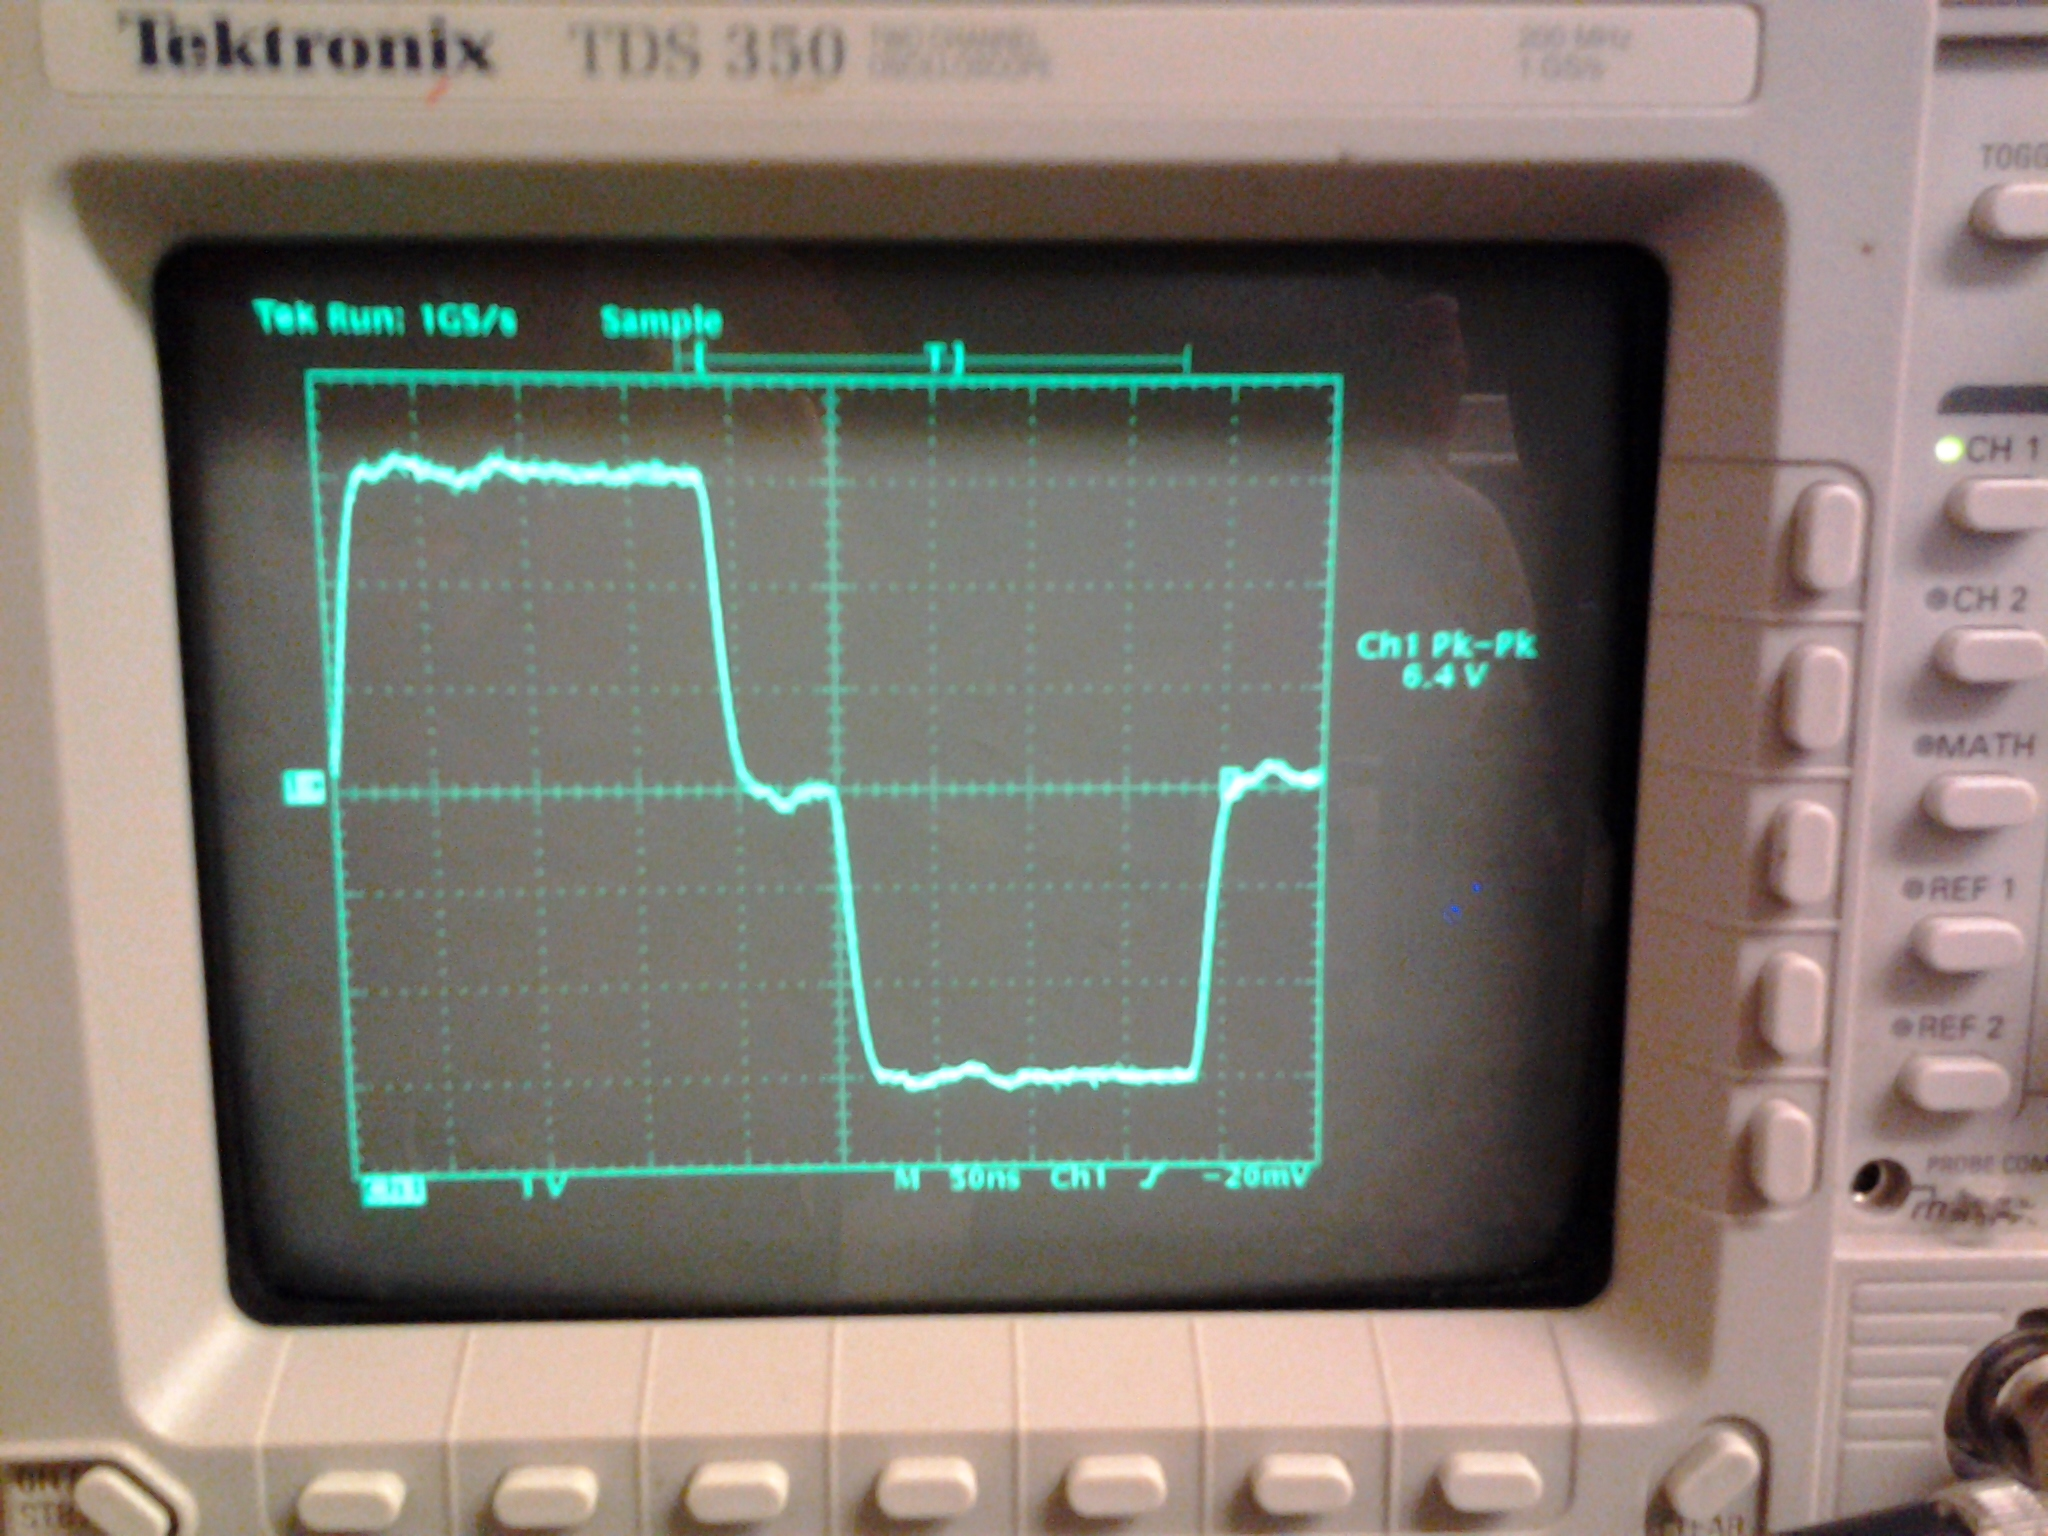
\includegraphics[scale=0.2]{reflection}
\caption{Superposition of incident and reflected waves in a cable \label{SUPER}}
%TODO: Obtain picture
\end{figure}
The final component $C_4$ serves the purpose of biasing, modifying the input for optimal
performance with our speaker system. As before, $C_4$ was fixed by our small selection of capacitors.
\begin{figure}
\centering
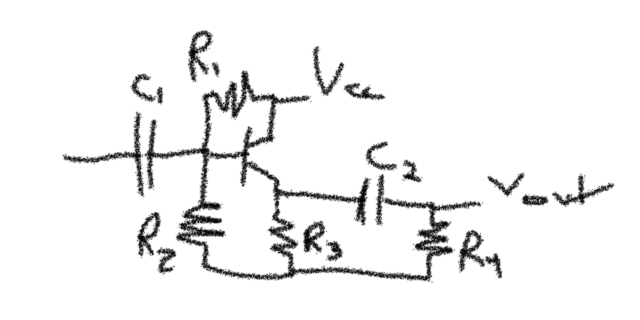
\includegraphics[scale=0.6]{ef}
$C_1 = 1 \mu$F$, C_2 = 1 \mu$F$, R_1 = 56$ k$\Omega, R_2 = 56$ k$\Omega, R_3 = 150\Omega, R_4 = 16$ k$\Omega, V_{cc} = 5$ V. 
\caption{Emitter Follower \label{EF}}
\end{figure}

In the second week of the lab, we learned about wave reflection and transmission-line termination, and we made
an amplifier. First, we put a square wave down a long cable, and we used careful oscilloscope measurements 
to detect the reflected wave. The image appears in Figure \ref{SUPER}. As you can see, the incident and reflected
waves have the same magnitude and opposite sign, but they are slightly out of phase so we get little stretches at the 
beginning and end of each period where they cancel each other. By measuring the extent of these stretches, 
we can get an idea of the propagation speed of the signal down the cable, since their length is the
amount of time it takes the signal to travel down the cable. Dividing this time, $3.6 * 10^{-9}$ seconds, into the length of
the cable, 6.2 meters, we get $1.9*10^8$ meters per second. When we put a $50\Omega$ resistor at the end of the 
cable, it was properly terminated, so the reflection no longer occured and all we saw was the square waveform, so
$50\Omega$ is the impedance of the cable. 

Then, we built an emitter-follower. A diagram of it appears in Figure \ref{EF}. An emitter-follower uses negative feedback
to cancel the amplification effects of the transistor. One noteworthy part of the circuit is the emitter resistor, 
the one directly below the output of the transistor. If this resistor were not present, the output of the transistor 
would be connected directly to ground, so $V_{out}$ would be 0. Instead, $V_{out} \approx V_{in}$ for an emitter.
Also, we found a bias voltage $V_{BE} \approx 0.73$ V. We predict that the emitter-follower would cease to operate properly
at around $V_{cc} - V_{BE} = 4.27$ V, but we never actually got around to measuring this voltage.

\begin{figure}
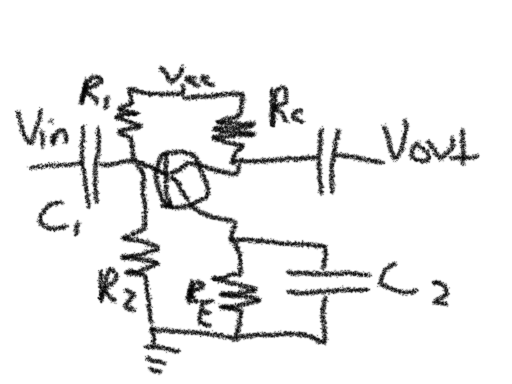
\includegraphics[scale=0.8]{amp}
\caption{Our FM Radio Amplifier \label{FMRA}}

$V_{cc} = 31.5 $V$, R_c = 510\Omega, R_E = 220\Omega, R_1 = 3900 \Omega, R_2 = 1006\Omega, C_1 = C_2 = 1\mu$F.
\end{figure}
Finally, we built our amplifier, which you can see in Figure \ref{FMRA}. $V_{cc}$ provides a DC input to the 
transistor, putting it into active mode in which it amplifies its AC input. $R_1$ and $R_2$ serve as a voltage
divider for the $V_{cc}$ power source, so that only a fraction of its voltage reaches the transistor; this
is necessary because the transistor only works with certain amplitudes of $V_{BE}$, and too much input will cause it 
to work improperly. Typical transistors work best with $V_{BE}$ around 0.7 V. Another important voltage is the base-collector
voltage, $V_{BC}$. This is a function of $V_{cc}$, $R_1, R_2, $ and $R_C$. If it gets too large, the transistor will shut
down, so it is one to be careful with. As in the
emitter-follower, $R_E$ increases the voltage at the emission terminal, allowing us to control the voltage difference
between the input and the emitter. With $R_E = 220\Omega$ as indicated in Figure \ref{FMRA}, we got $V_{BE} = 0.73$ V. $C_1$
does biasing for the circuit, modifying the phase of the input wave so that it works well with the transistor. 
$R_C$ affects the gain of the amplifier circuit by the formula $G = R_C / R_E$, where $G$ denotes the gain. 
$C_2$, the emitter capacitor, gives an additional resistance to the emitter terminal, one that decreases with increasing
frequency: as a result, the effective $R_E$ is lowered at these high frequencies and the gain increases.

The amplitude of the input voltage is added to $V_{BE}$, since it increases the voltage at the base. If $V_{BE}$ goes past about
one volt, the transistor becomes oversaturated and stops working properly. As such, we would expect the circuit to only work up to
an input amplitude of $.27$ V or so. As it turned out, we got reliable outputs up to around $.4$ V at 10 kHz. Two significant
aspects of such a circuit as this are the input and output impedances. The input impedance is the ratio of the input voltage
to the input current, and the output impedance is the ratio of $(V_{in} - V_{out}$ to the output current. When we were supplying 
.4 V at 10 kHz, we measured the input current as .03 A, as depicted in Figure \ref{current}.
\begin{figure}
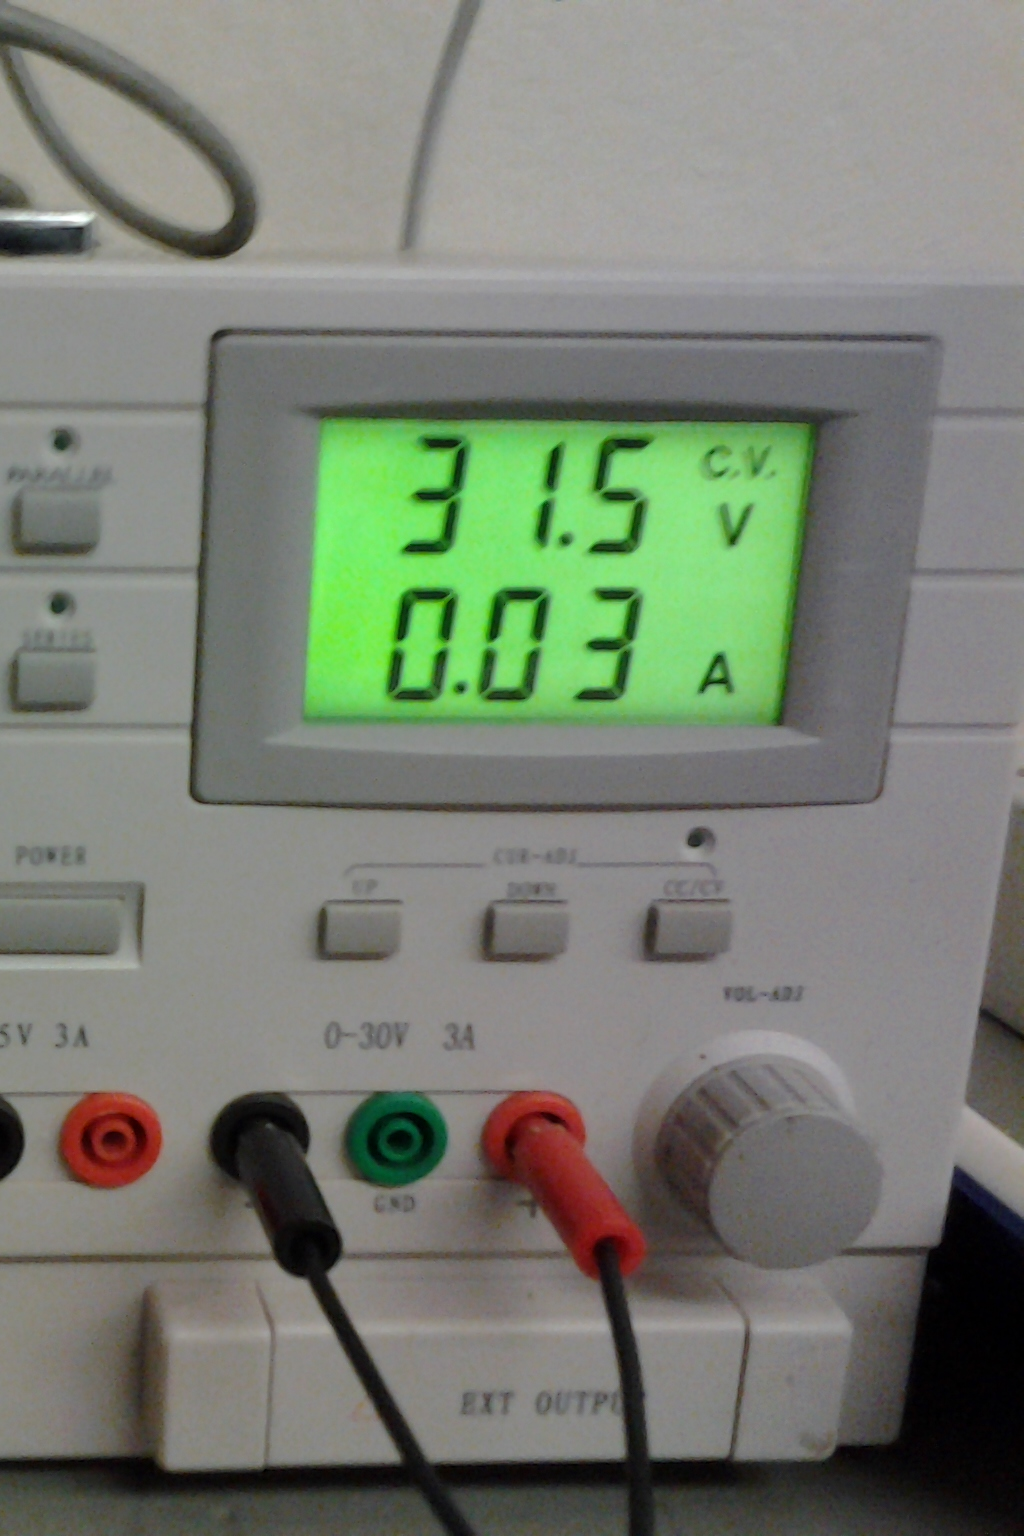
\includegraphics[scale=0.2]{right}
\caption{Our measurement of the input current (and $V_{cc}=31.5$ V)\label{current}}
\end{figure}
So the input impedance of our circuit is $.4/.03 = 13.3 \Omega$. Since we know the ratio $V_{out}/V_{in}$, which is the same
as the gain of the circuit $G = R_C / R_E = 2.3$, we can calculate the output impedance, even though we didn't measure the output
current: $Z_{out} = (V_{out} - V_{in}) / I_{out} = 1.3V_{in} / 2.3I_{in} = 1.3 / 2.3 * Z_{in} = 7.5 \Omega$.

If we were to connect our amplifier to an $8\Omega$ speaker by a long wire, we would terminate it with a 58$\Omega$ resistor.
This is because the wire has impedance $50 \Omega$ as we found before, and it is as though it is in series with the $8\Ohm$
speaker. With a $58\Omega$ resistor, we will not see reflections, so the signal quality will be better.

Earlier, I claimed that the gain of our amplifier circuit is $R_C / R_E$. However, this is only the low-frequency approximation,
which was relevant to the low frequencies used in the lab: in fact, the whole formula is
$G(\omega) = R_C / R_E * \sqrt{1 + R_E^2C_E^2\omega^2}$, where $\omega$ is the frequency of
the input signal. As such, at high frequencies such that $R_E^2C_E^2\omega^2 \approx 1$, we will
start to see the circuit diverge from its expected behavior. Solving for $\omega$, we find $\omega \approx 1.96$ MHz. Thus, the
operating band of our amplifier is on frequencies less than 1.96 MHz; above this frequency, it diverges from expected behavior.

In week 3, our goal was to observe Johnson-Nyquist noise on a resistor by amplifying it and measuring 
the amplified signal. The formula for the voltage generated by Johnson noise is
$V^2 = 4k_BTBR$, where $V$ is the voltage, $k_B$ is Boltzmann's constant, $T$ is the temperature
in Kelvins, $B$ is the bandwidth at which we are measuring, and $R$ is the resistance of the resistor
in question. Since we already built a $\approx 1$ MHz bandpass filter, I will use 1 MHz as the B-value in the calculation. 
For a 50$\Omega$ resistor at a warm room temperature of 300K,  $V = 9.1 * 10^{-7}$V. To amplify this to one mV for
detection, we would need a gain of $.001/(9.1 * 10^{-7}) \approx 1100$. Sadly, the lab's amplifiers mysteriously broke
before we had an opportunity to realize this experiment. No one knows why or how. As a result, we are unable to perform
measurements on the Johnson noise, since our measurement tools cannot detect a difference of $9.1*10^{-7}$ V. If we had
better measurement tools, perhaps we could make this measurement. Alternatively, we could try making the Johnson noise higher
by changing the temperature, bandwidth, or resistance. Unfortunately, the Johnson noise varies only as the square root
of these parameters, so with the available resistances and filters, if we stick to safe temperatures the Johnson noise
remains below the threshold of detection.

For instance, if we wanted to dissipate power through a resistor to increase its temperature, using $P = V^2 / R$ it would take
10 V to dissipate 2 W in a 50$\Omega$ resistor. By the Stefan-Boltzmann law, this would heat the resistor, which I'll approximate
as a blackbody with surface area $10^{-7}$ m, to $T = (P/(A\sigma))^{1/4} = 4333.7$ K. Actually assembling it, we measured the 
resistor temperature at 303 K, nowhere near the calculated value. This could be because the resistor is not a blackbody, 
my estimate of the area was bogus, the thermometer was playing tricks on me, or not all the energy dissipated in the resistor
went to heating it up. 

\begin{figure}
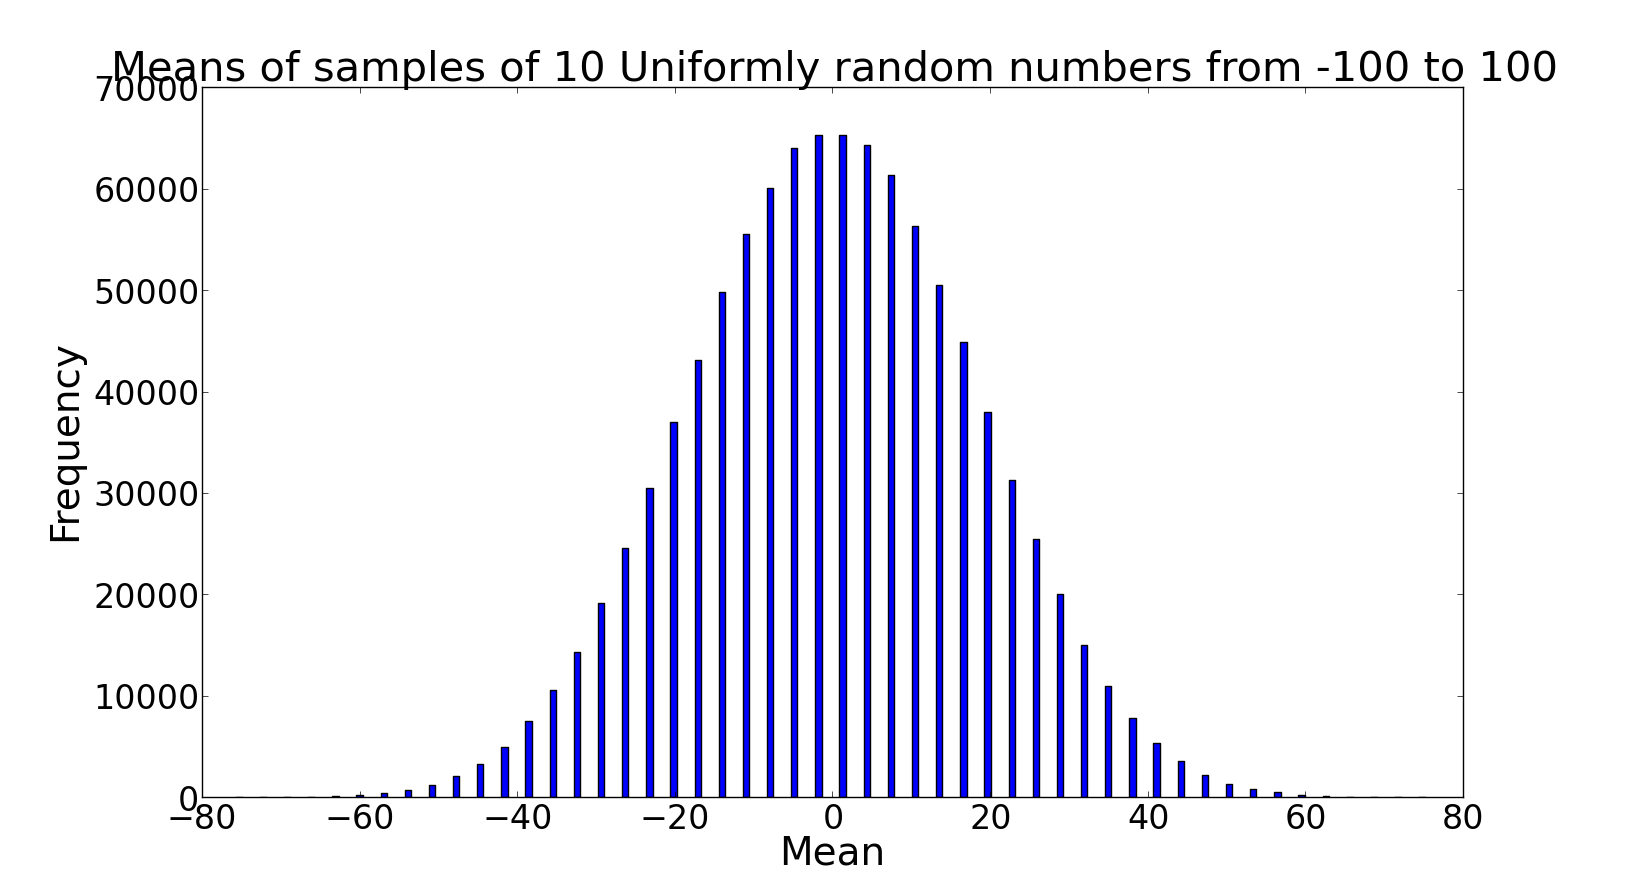
\includegraphics[scale=0.4]{centralimit}
\caption{Distribution of 1,000,000 sample means for samples drawn uniformly from (-100, 100) \label{centralimit}}
\end{figure}

In addition, the central limit theorem is cool and relevant. The central limit theorem states that if you sample any random distribution, 
take the mean of that sample, repeat that process several times, and plot the results, the resulting distribution of sample means is 
Gaussian, regardless of the underlying distribution from which the samples were originally taken. For instance, if you take a million
samples of ten uniformly random numbers between -100 and 100, the distribution of sample means is approximately Gaussian about 0. A
plot of just that appears in Figure \ref{centralimit}.

Also, the standard deviation of the distribution of sample means for samples of size $N$ decreases as $\sqrt{N}$. You can see this
in figure \ref{stdev}.

The noise figure of an amplifier is defined as $10\log{(\snrin/\snrout)}$, where $\snrin$ is the input signal-to-noise ratio and
$\snrout$ is the output signal-to-noise ratio. This measures the fraction of the output noise that is due to the components of 
the system, dividing out the noise that came into the system beforehand. To measure this with the technology we have, we would assume
that the Johnson noise is the only relevant input noise and divide the strength of the input signal by the amount of the
Johnson noise that we would have measured above to get the input signal-to-noise ratio. Then, we would measure the magnitude of the
output signal, and we would attempt to roughly approximate the strength of the output noise by oscilloscope divination. There are better 
tools for this, such as spectrum analyzers, but they weren't in the budget apparently. This gives us the output signal-to-noise
ratio, and by taking 10 times the log of our ratios we would arrive at the noise figure. Sadly, we had no amplifiers, so we did
not get the privilege of doing all that.

Finally, there's this thing called an Allan variance test. Basically, if you're trying to measure a value accurately, you will want to measure it many
times. As noise affects your measurements, you may get differing values every time. So let's say you have a hundred measurements,
$x_k$ for $k \in [1, 100]$. To run an Allan variance test, you first calculate $1/2*\sum_{k=2}^{100}(x_{k+1}-x_k)^2$. This is $\sigma_x^2(1)$,
where $\sigma_x^2$ is the Allan variance function. Then, you divide the data into 50 groups of 2, take the mean $y_l$ of each of
those groups, and compute $1/2 * \sum_{k=2}^{50}(y_{k+1}-y_k)^2$ to get $\sigma_x^2(2)$. You continue in this way until you've 
partitioned the data into one group of 100, at which point you have every available value of $\sigma_x^2$. This generates
a plot of variances versus number of samples averaged that you can interpret to determine the timescales of various noise
sources in your experiment. A plot of Allan variance for 1000 random numbers is included in Figure \ref{allan}. This one shows
no discernible relationship between sample size and variance. 

\begin{figure}
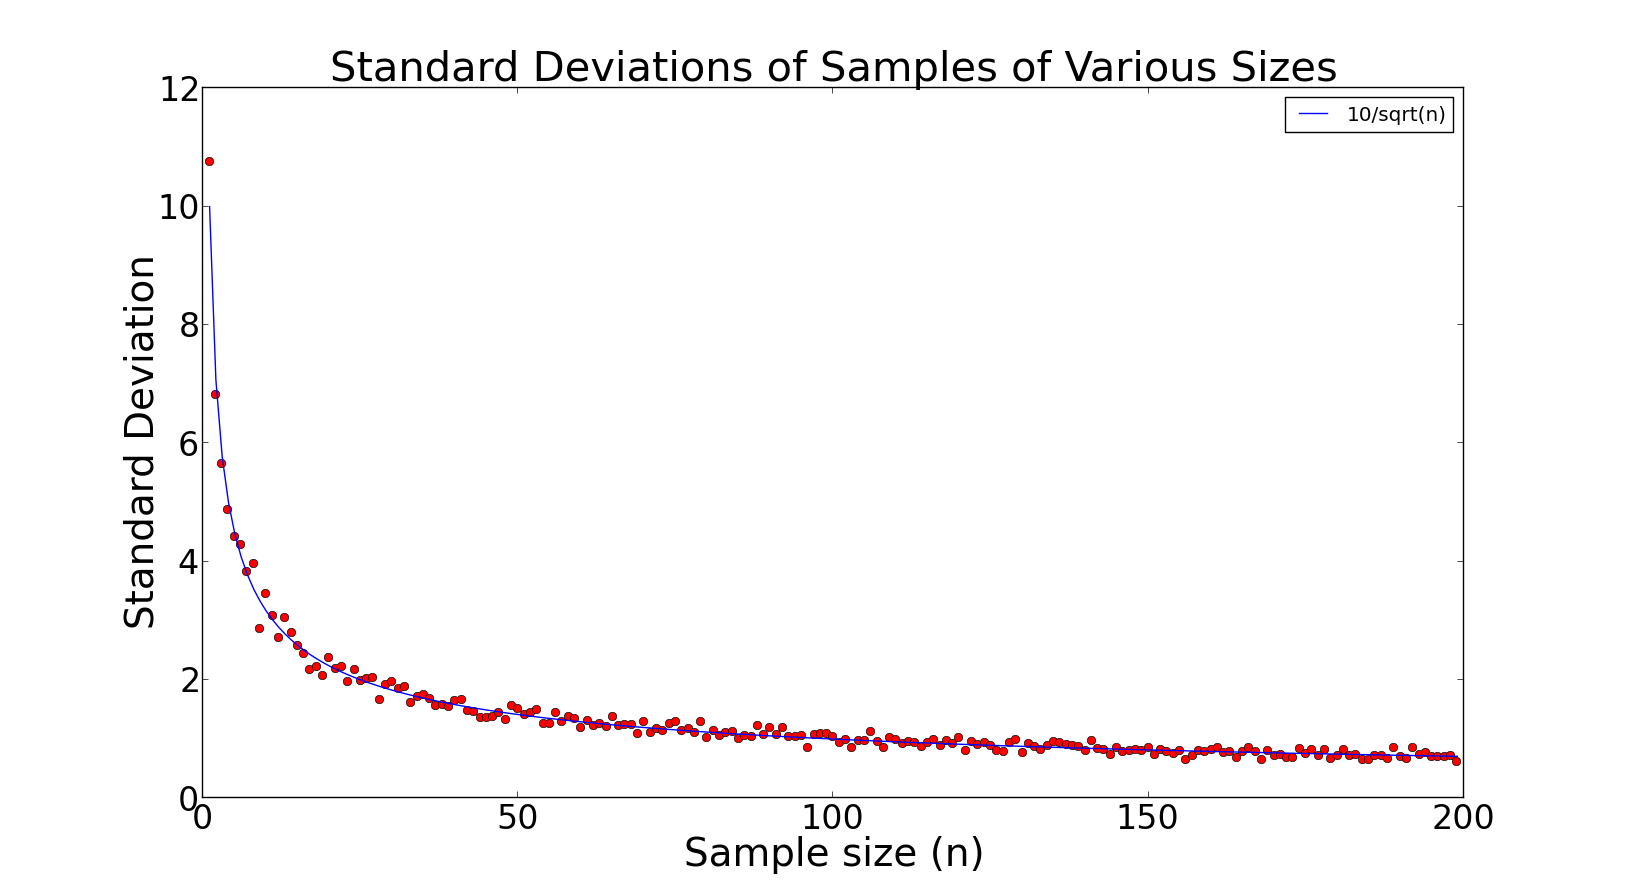
\includegraphics[scale=0.4]{stdev}
\caption{Standard deviation of distributions of sample means for various sample sizes \label{stdev}}
\end{figure}

\begin{figure}
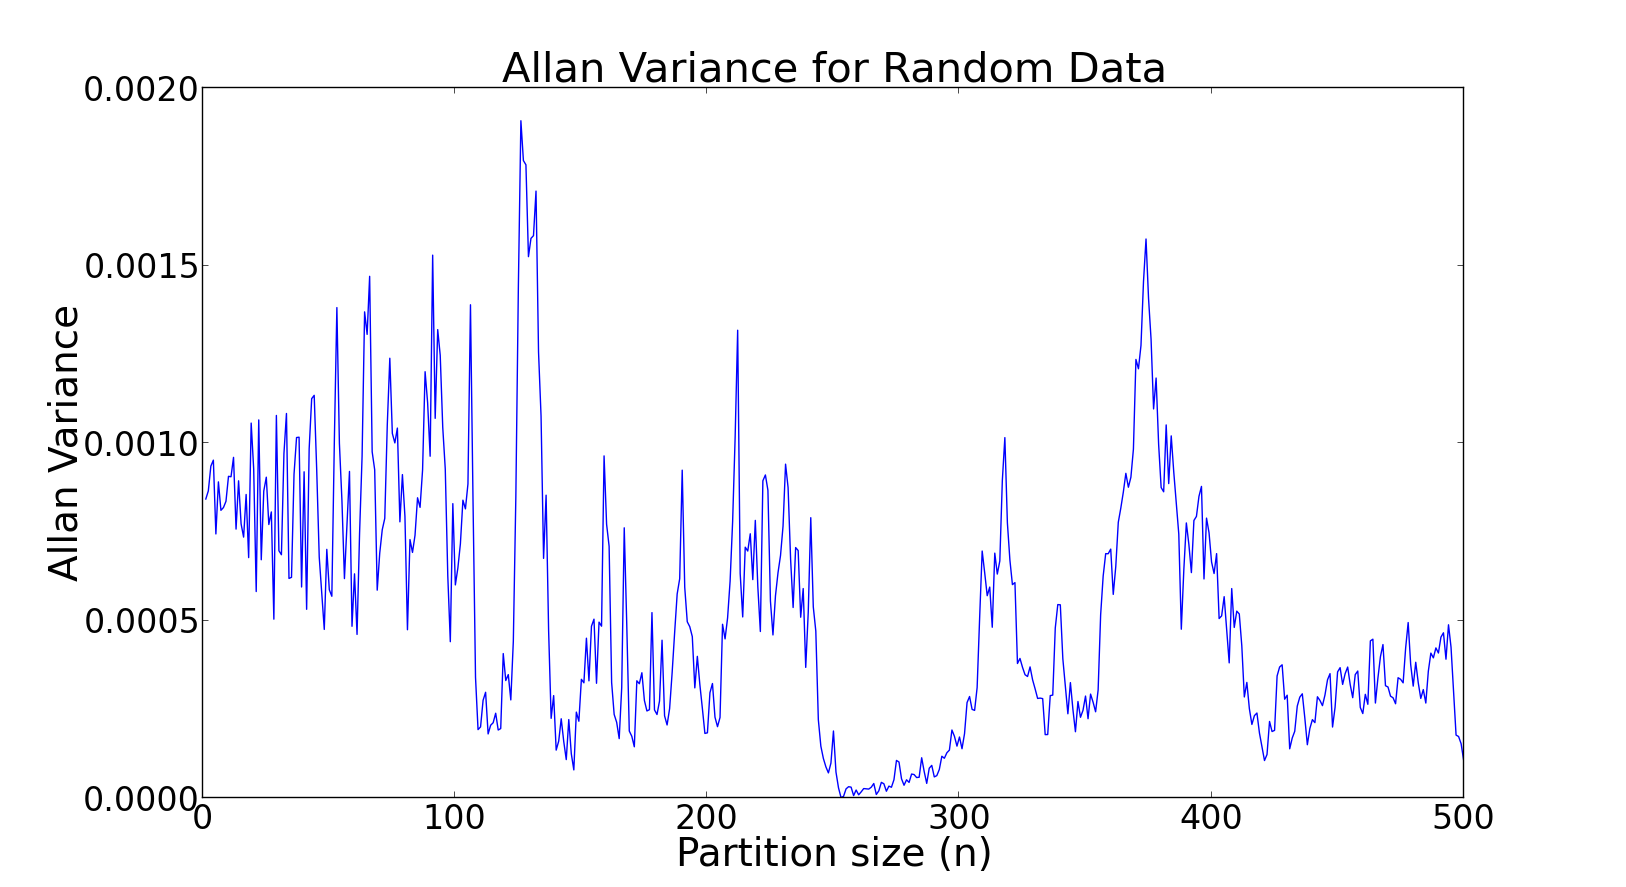
\includegraphics[scale=0.4]{allan}
\caption{Allan Variance for a group of 1000 random numbers \label{allan}}
\end{figure}

\section{Conclusion}
In conclusion, this was a very interesting lab. We built many cool electronics, and I learned a lot about circuits and radios and Allan variation.
All circuits I build from now on involving transmission lines will be properly terminated, so there will be no reflection errors. With my new 
knowledge of transistor operation, I can design and implement cool transistor circuits to perform any of the many functions of a transistor.
If we could return with some functioning amplifiers, we could make Part 3 work in its entirety and really see Johnson noise. Indeed, this lab
laid the foundation for some really great physics work later!
\pagebreak
\section{Works Cited}
\begin{enumerate}
\item\url{http://hyperphysics.phy-astr.gsu.edu/hbase/electric/filter.html#c1} reminded me about filters and their transfer functions.
\item\url{http://www.cirvirlab.com/index.php/tutorials/88-npn-bjt-common-emitter-amplifier.html} explained how NPN BJT amplifiers work. 
\item\url{http://www.phidgets.com/docs/Allan_Deviation_Primer} and \url{http://en.wikipedia.org/wiki/Allan_variance} taught me about Allan variance testing.
\end{enumerate}
\end{document}

\section{Acknowledgements}
My lab partners for this lab were Leo and Isaac. They did a really great job!
